%; whizzy chapter
% -initex iniptex -latex platex -format platex -bibtex jbibtex -fmt fmt

%   Pdf作成手順
% dvipdfmx debianmeetingresume2005-natsu.dvi


%     Tokyo Debian Meeting resources
%     Copyright (C) 2006 Junichi Uekawa

%     This program is free software; you can redistribute it and/or modify
%     it under the terms of the GNU General Public License as published by
%     the Free Software Foundation; either version 2 of the License, or
%     (at your option) any later version.

%     This program is distributed in the hope that it will be useful,
%     but WITHOUT ANY WARRANTY; without even the implied warranty of
%     MERCHANTABILITY or FITNESS FOR A PARTICULAR PURPOSE.  See the
%     GNU General Public License for more details.

%     You should have received a copy of the GNU General Public License
%     along with this program; if not, write to the Free Software
%     Foundation, Inc., 51 Franklin St, Fifth Floor, Boston, MA  02110-1301 USA


%この資料はA3用紙に一面あたり2頁両面印刷(一枚で4頁)で印刷する予定
\documentclass[mingoth,a4paper]{jsarticle}
\usepackage[dvipdfmx]{graphicx}
\usepackage{fancybox}
\usepackage{longtable}
\usepackage{ascmac}	% 囲み (screen,itembox)
\usepackage{fancyvrb}   % 囲み Verbatim のために必要
\usepackage[dvipdfmx]{hyperref}
\usepackage{url}

%http://www.naney.org/diki/dk/hyperref.html
%日本語EUC系環境の時
\AtBeginDvi{\special{pdf:tounicode EUC-UCS2}}
%シフトJIS系環境の時
%\AtBeginDvi{\special{pdf:tounicode 90ms-RKSJ-UCS2}}

%% spacing の設定をする。枠を減らす。 89->77頁に減った。
\setlength\headheight{0mm}
\setlength\topmargin{-20mm}
\setlength\headsep{0mm}
\setlength\topskip{3mm}
\setlength\maxdepth{4pt}
\setlength\columnsep{6mm}
\setlength\textheight{252mm}
\setlength\topmargin{-5mm}
\setlength\textwidth{170mm}
\setlength\oddsidemargin{-5mm}
\setlength\evensidemargin{-5mm}


% とりあえずcommandline環境を定義。入出力についてはcommandline環境を活用
%する
\newenvironment{commandline}%
{\VerbatimEnvironment
  \begin{Sbox}\begin{minipage}{15cm}\begin{fontsize}{7.3}{7.3} \begin{BVerbatim}}%
{\end{BVerbatim}\end{fontsize}\end{minipage}\end{Sbox}
  \setlength{\fboxsep}{8pt}\fbox{\TheSbox}}



% 三択問題用
\newcounter{santakucounter}
\newcommand{\santaku}[4]{%
\addtocounter{santakucounter}{1}

\nopagebreak 問題\arabic{santakucounter}. 
#1\\
\nopagebreak□ A #2\\
\nopagebreak□ B #3\\
\nopagebreak□ C #4
\pagebreak[1]
\hspace{1cm}
\\

}

\newcommand{\emptyspace}{(\underline{\hspace{1cm}})}



\newcommand{\subsubsubsection}[1]{%
\vspace{1zw}{\bf #1}\\}


% sectionをセンタリングする
\makeatletter
  \renewcommand{\section}{\@startsection{section}{1}{\z@}%
    {\Cvs \@plus.5\Cdp \@minus.2\Cdp}% 前アキ
    {.5\Cvs \@plus.3\Cdp}% 後アキ
    {\normalfont\Large\headfont\raggedright\centering}} % style
\makeatother

% section の代わりの環境
\newcommand{\dancersection}[2]{%
\newpage
東京エリアDebian勉強会 2005 夏
\hrule
\vspace{0.5mm}
\hrule
\hfill{}
\includegraphics[width=3cm]{image200502/openlogo-nd.eps}\\
\vspace{-4cm}
\begin{center}
  \section{#1}
\end{center}
\hfill{}#2\hspace{3cm}\space\\
\hrule
\hrule
\vspace{1cm}
}




%% for gotom
\newenvironment{gdescription}%  
{%
   \begin{list}{}% 見出し記号/直後の空白を調節
   {%
      \setlength{\itemindent}{0mm}
      \setlength{\leftmargin}{45mm}%  左のインデント
      \setlength{\rightmargin}{0zw}% 右のインデント
      \setlength{\labelsep}{4mm}%    黒丸と説明文の間
      \setlength{\labelwidth}{4cm}%  ラベルの幅
      \setlength{\itemsep}{0em}%     項目ごとの改行幅
      \setlength{\parsep}{0cm}%      段落での改行幅
      \setlength{\listparindent}{0cm}% 段落での一字下り
      \let\makelabel\gdescriptionlabel
   }
}{%
   \end{list}%
}
\newcommand*\gdescriptionlabel[1]{\hspace\labelsep\normalfont\bfseries #1}
%%

\begin{document}

\begin{titlepage}

% 毎月変更する部分
\title{%
\includegraphics[width=9cm]{image200502/openlogo-nd.eps}\\
あんどきゅめんてっどでびあん}
\date{}
\author{\bf 東京エリアDebian勉強会} 
%\maketitle  % use the graphics instead of the text

\includegraphics[height=252mm]{image200508/titlepage3.eps}
%\thispagestyle{empty}
\end{titlepage}

\newpage
\setcounter{tocdepth}{1}
\tableofcontents
\vspace{6cm}

\large
\begin{itembox}{\bf『あんどきゅめんてっど でびあん』について}
本書は、東京周辺で毎月行なわれている『東京エリア Debian 勉強会』で
使用された資料・小ネタ・必殺技などを一冊にまとめたものです。
収録範囲は勉強会第1回〜第6回まで。
内容は無保証、つっこみなどがあれば勉強会にて。
\end{itembox}
\normalfont

\dancersection{Debian Social Contractについて}{松山}

\subsection{Debian Social Contractって何だ?}
Debian プロジェクト憲章 (v1.2)より\footnote{\url{http://www.debian.org/devel/constitution}}
\begin{itemize}
\item「基本文書 (Foundation Document)」とは,Debianプロジェクトの使命や目的にとって決定的に重要とみなされる文書または声明である.
\item「基本文書」は,「Debian社会契約(Debian Social Contract)」
および「Debianフリーソフトウェアガイドライン (Debian Free Software Guidelines)」というタイトルの文書である.
\item「基本文書」を更新するためには,3:1 の多数決を必要とする.
新たな「基本文書」の発行や既存の「基本文書」の撤回は,この憲章のリストを修正することによってなされる.
\end{itemize}
国なら憲法,DebianにはSocial Contractといったところでしょうか.

\subsubsection{「Debian は 100\% フリーソフトウェアであり続けます.」}
Debianプロジェクトは社会契約において
Debian GNU/Linuxディストリビューションを完全にフリーな ソフトウェアとして維持する
ことを約束しています.
フリーソフトウェアとはどういうソフトウェアなのか,というのはDebian Free Software Guidline(DFSG)で記述されています.

\subsubsection{「私たちはフリーソフトウェアコミュニティーにお返しをします.」}
DSCには
\begin{quote}
私たちのシステムに含まれているソフトウェアを私たちの「上流」で開発している作者に,バグ修正,改良,ユーザの要求などをフィードバックします.
\end{quote}
とありあます.最近MLにDebianデベロッパー同士で「もっと上流の人と密にコミュニケーションとろうよ」的な投稿がありました.実際のところはどうなのでしょうか.

\subsubsection{「私たちは問題を隠しません.」}
プロジェクトに報告されているバグは全て参照できます.
Debianでは開発者間,ユーザ間のやりとりのほとんどがメーリングリストを通して行われるそうです.
Debianはバグの情報に関することのみならず,プロジェクトに関するいろんなことを公開しているようです.

\subsubsection{「私たちはユーザとフリーソフトウェアを大切にします.」}
DSCには
\begin{quote}
私たちはユーザーとフリーソフトウェアコミュニティからの要求に従います.
彼らの関心と利益を最優先に考えます.
私たちはさまざまな状況におけるコンピュータ利用環境の運用に関してユーザーの必要を満たすように行動します.
\end{quote}
とあります.BTSに「要望」という重要度が用意されているところに,こういった姿勢が現われているでしょうか.

\subsubsection{「私たちのフリーソフトウェア基準に合致しないプログラムについて.」}
Debianプロジェクトは
\begin{quote}
私たちは,Debianフリーソフトウェアガイドラインに適合していないプログラムを使わなければならないユーザーがいることを認めています.
\end{quote}
最初の社会契約との折り合いからか,Debianパッケージアーカイブにはmain,contrib,non-freeというカテゴリを作成し,パッケージを整理しています.

\subsection{Debianニュースに見るDebianの思想}
拒否: Debian プロジェクトは Sender ID を採用できません\footnote{\url{http://www.debian.org/News/2004/20040904}}
\begin{quote}
...省略...
また私たちは,インターネットの核となるインフラストラクチャに関する知的財産権 (IPR) は企業に対して認められるべきではないと考えています.IETF が IPR に関するポリシーを見直し,インターネットの核となるインフラストラクチャが妨げられないよう保証する必要があると信じています.
...省略...
\end{quote}
Debian セキュリティ勧告は CVE と互換性があります\footnote{\url{http://www.debian.org/News/2004/20040330}}
\begin{quote}
...省略...
公に知られた脆弱性およびセキュリティ上の問題点のすべてについて名前を標準化することを目的とするCommon Vulnerabilities and Exposures (CVE) プロジェクトとの協調的な取り組みの中で, 2002 年 6 月以来,新たなセキュリティ勧告は CVE 識別番号を含めた形で出されています. Debian は 2003 年 5 月に 正式に CVE との互換性を申請しました.
...省略...
\end{quote}
Debian はデスクトップ Linux コンソーシアムに参加します\footnote{\url{http://www.debian.org/News/2003/20030207}}
\begin{quote}
Debian プロジェクトは,最近設立され,非営利法人になる予定の デスクトップ Linux コンソーシアム (DLC) の設立メンバーです.
...省略...
Debian デスクトップ サブプロジェクトは,デスクトップ用途に GNU/Linux を利用しているユーザのために Debian の改善に精力を傾け続けている一例です.
...省略...
\end{quote}

\dancersection{debhelper論 その1 Debhelperとは何か。存在意義は何か。}{上川}

\subsection{Debian packageの構成要件}


Debian Packageのソースパッケージには下記ファイルが必要です。
全てのファイルについては規定のフォーマットがあります。

\begin{itemize}
 \item debian/rules: パッケージをビルドする手順を記述したMakefile.
 \item debian/control: パッケージの情報を記述した構成ファイル
 \item debian/copyright: パッケージの著作権情報を記述したファイル。利用
       許諾を記述。
 \item debian/changelog: 変更履歴を記述する。
\end{itemize}


emacsで編集するのであれば、devscripts-elパッケージをインストールすると
編集しやすくなっています。
vi を利用しているのであれば、devscriptsパッケージを利用すると、
各ファイルを編集しやすいです。


パッケージの作成の本質は、ディレクトリ以下にアプリケーションをインストー
ルし、
それ以下のファイルをtarでかためて、debファイルのなかにいれることです。
その他に制御情報もありますが、それについては後日。

例えば、debian/tmp/以下に / 以下にインストールされるはずのファイルを配置
することでパッケージを作成できます。
debian/tmp/usr/bin/binary-test
というファイルを作成して、debian/tmpディレクトリを指定してdpkg-debコマン
ドを実行してできたパッケージをインストールしたら/usr/bin/binary-test
にファイルがインストールされます。


\subsection{dh-make}

アップストリームからのソースパッケージから、Debian用のパッケージのテンプ
レートを作成します。

さて、dh-make ではどんなファイルが作成されるのでしょうか。

なんでもないサンプルファイルを作成して試しに実行してみます。

\begin{commandline}
	
[02:11:56]ibookg4:/tmp/dh> find -ls 
 94712    0 drwxr-xr-x   3 dancer   dancer         80  1月 27 02:08 .
 94686    4 -rw-r--r--   1 dancer   dancer        156  1月 27 02:07 ./test-source_0.1.orig.tar.gz
 94672    0 drwxr-xr-x   2 dancer   dancer         60  1月 27 02:07 ./test-source-0.1
 94675    0 -rw-r--r--   1 dancer   dancer          0  1月 27 02:07 ./test-source-0.1/Makefile
\end{commandline}

dh-make コマンドをうつと、どんなバイナリを作成するのか、という点を聞かれ
ます。

\begin{commandline}
	
[02:13:42]ibookg4:/tmp/dh/test-source-0.1> dh_make

Type of package: single binary, multiple binary, library, or kernel module?
[s/m/l/k] s

Maintainer name : Junichi Uekawa
Email-Address   : dancer@debian.org 
Date            : Thu, 27 Jan 2005 02:13:46 +0900
Package Name    : test-source
Version         : 0.1
Type of Package : Single
Hit <enter> to confirm: 
Done. Please edit the files in the debian/ subdirectory now. You should also
check that the test-source Makefiles install into $DESTDIR and not in / .
[02:13:51]ibookg4:/tmp/dh/test-source-0.1> 
\end{commandline}


\begin{commandline}

[02:27:24]ibookg4:/tmp/dh/test-source-0.1> ls debian/
README.Debian  dirs		   manpage.sgml.ex  rules
changelog      docs		   manpage.xml.ex   test-source-default.ex
compat	       emacsen-install.ex  menu.ex	    test-source.doc-base.EX
conffiles.ex   emacsen-remove.ex   postinst.ex	    watch.ex
control        emacsen-startup.ex  postrm.ex
copyright      init.d.ex	   preinst.ex
cron.d.ex      manpage.1.ex	   prerm.ex
\end{commandline}

大量にファイルができます。これらのファイルで、.exで終了しているのはサン
プルファイルで、特に必要でないのなら削除します。


debian/rulesとして、次のようなファイルができます。

\begin{commandline}
#!/usr/bin/make -f
# -*- makefile -*-
# Sample debian/rules that uses debhelper.
# This file was originally written by Joey Hess and Craig Small.
# As a special exception, when this file is copied by dh-make into a
# dh-make output file, you may use that output file without restriction.
# This special exception was added by Craig Small in version 0.37 of dh-make.

# Uncomment this to turn on verbose mode.
#export DH_VERBOSE=1




CFLAGS = -Wall -g

ifneq (,$(findstring noopt,$(DEB_BUILD_OPTIONS)))
	CFLAGS += -O0
else
	CFLAGS += -O2
endif

configure: configure-stamp
configure-stamp:
	dh_testdir
	# Add here commands to configure the package.

	touch configure-stamp


build: build-stamp

build-stamp: configure-stamp 
	dh_testdir

	# Add here commands to compile the package.
	$(MAKE)
	#docbook-to-man debian/test-source.sgml > test-source.1

	touch build-stamp

clean:
	dh_testdir
	dh_testroot
	rm -f build-stamp configure-stamp

	# Add here commands to clean up after the build process.
	-$(MAKE) clean

	dh_clean 

install: build
	dh_testdir
	dh_testroot
	dh_clean -k 
	dh_installdirs

	# Add here commands to install the package into debian/test-source.
	$(MAKE) install DESTDIR=$(CURDIR)/debian/test-source


# Build architecture-independent files here.
binary-indep: build install
# We have nothing to do by default.

# Build architecture-dependent files here.
binary-arch: build install
	dh_testdir
	dh_testroot
	dh_installchangelogs 
	dh_installdocs
	dh_installexamples
#	dh_install
#	dh_installmenu
#	dh_installdebconf	
#	dh_installlogrotate
#	dh_installemacsen
#	dh_installpam
#	dh_installmime
#	dh_installinit
#	dh_installcron
#	dh_installinfo
	dh_installman
	dh_link
	dh_strip
	dh_compress
	dh_fixperms
#	dh_perl
#	dh_python
#	dh_makeshlibs
	dh_installdeb
	dh_shlibdeps
	dh_gencontrol
	dh_md5sums
	dh_builddeb

binary: binary-indep binary-arch
.PHONY: build clean binary-indep binary-arch binary install configure
\end{commandline}


また、debian/controlとして下記のようなファイルができます。

\begin{commandline}
Source: test-source
Section: unknown
Priority: optional
Maintainer: Junichi Uekawa <dancer@debian.org>
Build-Depends: debhelper (>= 4.0.0)
Standards-Version: 3.6.1

Package: test-source
Architecture: any
Depends: ${shlibs:Depends}, ${misc:Depends}
Description: <insert up to 60 chars description>
 <insert long description, indented with spaces>

\end{commandline}

他に必要なファイルとして、debian/changelogなどがあります。

\subsection{dh-xxxx のオーバビュー}

各論に入るまでにdh-xxxxが一般的にどういう動作を
するものなのかを説明します。おおざっぱにいうと二種類の動作形態があります。

Debian パッケージを作成する一連の動作の中で、
{\tt debian/パッケージ名 }
というディレクトリにインストール用のイメージを作成します。
そのディレクトリに対して、
{\tt debian/機能.パッケージ名 }
というファイルで指定した内容を実施してくれるのが
{\tt dh-機能} スクリプトです。

また、別の機能として、
コマンドラインオプションに指定されたものに対しても操作します。

\subsection{簡単なところから, dh-installman}

man ページをインストールするdh-installmanを例にとって、説明します。

man ページは各パッケージのセクションに応じたディレクトリにインストールし
ます。
セクション情報は、manページのroffソースの最初のところに記述してあります。

例\\

{\tt .TH "pbuilder" \underline{\it 8} "2004 Apr 4" "Debian" "pbuilder" }

このmanページはセクション8のマニュアルなので、FHSに従い、
{\tt /usr/share/man/man8/}というディレクトリにインストールする
必要があります。

下記の実行例は、インストール対象のパッケージ名を指定して、インストールす
るファイルを指定した場合です。

\begin{commandline}
 dh_installman -ppbuilder-uml pbuilder-user-mode-linux.1 \
 pbuilder-uml.conf.5 pdebuild-user-mode-linux.1
\end{commandline}

上記のコマンドを入力すると

{\tt debian/pbuilder-uml/usr/share/man/man1/pbuilder-user-mode-linux.1}
などにファイルがコピーされます。

debhelperの概念で重要なのは、このインストール先のディレクトリがどこであ
るかという
ことについてはdebhelper側で管理しており、
たとえポリシーに変更が発生しても、debhelperのみを変更すればよく、
パッケージスクリプト側への変更は最小にできる、という点です。

例えば、マニュアルページの例でいくと、
以前の標準では、/usr/man/man1/などにインストールすることがポリシーだった
のですが、それが変更になり、/usr/share/man/man1になりました。

\dancersection{debhelper論 その2 Debhelperの各コマンドは何者か。}{上川}

\subsection{debhelperコマンド編}


全体を見渡すために、debhelper 4.2.31に含まれているコマンドの一覧を表にしてみます。

ここでインストールといっているのは、ファイルをパッケージビルド用のディレ
クトリにコピーする、という意味です。

debian/packagename 
というディレクトリ以下にコピーすることにより、builddebの際にdebファイル
にコピーされ、後にインストールできるようになります。

DEBIANディレクトリというのは、
debian/packagename/DEBIAN
のことで、後にdpkgファイルのcontrol.tar.gzになる部分です。



%\begin{table}[h]
\begin{longtable}{|p{3cm}|p{7cm}|p{5cm}|}
\hline
\hline
名称 & 入力ファイル & 効能\\
\hline
\hline
builddeb & & .debファイルを作成 \\
\hline
clean & & 不要なファイルを消す debian/rules clean 用 \\
\hline
compress & package.compressスクリプト & ドキュメントの圧縮 \\
\hline
desktop & & .desktopファイルの登録\\
\hline
fixperms & & ファイル権限の修正\\
\hline
gconf & & gconf schemaの登録 \\
\hline
gencontrol & & dpkg-gencontrolのラッパ。 controlファイルをDEBIANディレク
 トリにインストール \\
\hline
install & package.install & ファイルをインストールする \\
\hline
installcatalogs & package.sgmlcatalogs & SGMLカタログを登録 \\
\hline
installchangelogs & & ChangeLogをインストールする \\
\hline
installcron & package.cron.monthly, package.cron.weekly,
 package.cron.daily package.cron.hourly package.cron.d  & cronスクリプト
 をインストール \\
\hline
installdeb & & DEBIANディレクトリにファイルをインストール \\
\hline
installdebconf & package.config package.templates & debconf用のファイル
 をインストール \\
\hline
installdirs & package.dirs & ディレクトリを作成 \\
\hline
installdocs & package.docs & ドキュメントをインストール \\
\hline
installemacsen & package.emacsen-install package.emacsen-remove
 package.emacsen-startup & emacs用スクリプトをインストール \\
\hline
installexamples & package.examples & example ファイルをインストールする \\
\hline
installinfo & package.info & infoをインストールする \\
\hline
installinit & package.init package.default & initスクリプトをインストー
 ルする。defaultファイルをインストールする。 \\
\hline
installlogcheck &  debian/package.logcheck.cracking
 debian/package.logcheck.violations
 debian/package.logcheck.violations.ignore
 debian/package.logcheck.ignore.workstation
 debian/package.logcheck.ignore.server
 debian/package.logcheck.ignore.paranoid & logcheck用のスクリプトを登録 \\
\hline
installlogrotate & package.logrotate & logrotate用のスクリプトを登録 \\
\hline
installman & package.manpages & manをインストール\\
\hline
installmanpages & & installmanを使いましょう   \\
\hline
installmenu & package.menu & メニューを追加 \\
\hline
installmime & debian/package.mime debian/package.sharedmimeinfo &
 mime情報を追加 \\
\hline
installmodules & debian/package.modules debian/package.modprobe &
 modutilでmoduleを追加 \\
\hline
installpam & debian/package.pam & PAM設定ファイルのインストール \\
\hline
installppp & debian/package.ppp.ip-up debian/package.ppp.ip-down & ppp
 設定ファイルのインストール \\
\hline
installwm & & Window managerを update-alternativesに登録\\
\hline
installxfonts & & X フォントの登録 \\
\hline
link & package.links & シンボリックリンクの作成 \\
\hline
listpackages &  & 処理するパッケージの一覧を出力するだけ \\
\hline
makeshlibs & & shlibsファイルを生成する \\
\hline
md5sums & & DEBIAN/md5sumsファイルを生成する \\
\hline
movefiles & & installを使ってください。 \\
\hline
perl & & perlスクリプトの依存関係を自動生成する \\
\hline
python & & pythonモジュールの依存関係の自動生成と、プリコンパイルのため
 のpre/postinstスクリプトの自動生成 \\
\hline
scrollkeeper & & OMFファイルの登録 \\
\hline
shlibdeps & & 共有ライブラリ依存関係情報の自動取得 \\
\hline
strip & & デバッグ情報のstrip \\
\hline
suidregister & & もう使わないでください \\
\hline
testdir & & 正しいディレクトリにいることを確認してくれる \\
\hline
testroot & & root権限で実行されていることを確認 \\
\hline
testversion & & debhelperのバージョンを確認する。今後はBuild-Dependsで指
 定してください。 \\
\hline
undocumented & & もう使わないでください \\
\hline
usrlocal & & /usr/local以下のディレクトリに関してポリシに基づいた作成/削除を実
 施。\\
\hline
\hline
\end{longtable}


\subsubsection{dh-testroot}

debian/rules スクリプトの中で、Policyで定義されている
「実行にはroot権限が必要」となっている部分があります。
本当にroot権限で実行されているのか確認してあげる部分です。

{\tt id -u}  コマンドの出力が 0であるか、とか
{\tt whoami }コマンドの出力が rootであるか、とかで確認します。
fakerootで実行されることが多いため、fakerootでだまし切れる内容にする必要があります。

今後selinuxなどの広がりにより、rootである、ということのチェックだけでは
不十分になったばあいには
debhelper側で機能が拡張されることでしょう。

\subsubsection{dh-testdir}

現在のディレクトリが、debianパッケージのソースディレクトリであるか、とい
うことを確認します。
ここでは、カレントディレクトリからみて、./debian/rulesというファイルが存
在するか、
などということで確認できます。

\subsubsection{dh-clean}

作業用に利用したファイルを消します。
インストールイメージを作成するために一時的に作成する
{\tt debian/パッケージ名 } ディレクトリの削除はここで実行します。




\newpage
%\vfill{}
%\hfill{}
%
\includegraphics[width=7cm]{image200502/openlogo-nd.eps}
%\hfill{}
%\vfill{}
%\newpage

\dancersection{debhelper論 その3 Debhelperの処理の流れ。}{上川}

\subsection{debhelperの実行フロー}

debhelperの一般的な実行フローにおいてどのファイルがどういう順番でコピー
されていくのか、という部分について追跡してみます。

\subsubsection{debian/rules clean}

debhelperとしては、Debianパッケージのビルドに利用した一時ファイルを削除
します。

debian/以下のディレクトリの削除を実施します。
\begin{itemize}
 \item {\it packagename} ディレクトリ
 \item  {\it packagename}*.debhelper
 \item files
 \item tmp
\end{itemize}

また、一般的な一時ファイルの削除も実施します。
\begin{itemize}
 \item \verb!#*#!
 \item \verb!*~!
 \item DEADJOE
 \item *.orig
 \item *.rej
 \item *.bak
 \item *.SUMS
 \item TAGS
 \item core
 \item */.deps/*.P
 \item auotm4te.cache
\end{itemize}


\subsubsection{debian/rules build}

ここでは、debhelperはほとんどなにもしません。
上流のソースコードに対してMakeし、コンパイルする作業が主です。

カレントディレクトリが正しい場所か、ということを
確認します。

\subsubsection{debian/rules install}

ここでは、debhelperを利用して、インストール先のディレクトリを作成し、
そのディレクトリにソフトウェアをインストールします。

dh\underbar{ }installdirsで、必要なディレクトリを
{\tt debian/{\it package}}
以下に作成します。

{\tt debian/{\it package}}
ディレクトリににソフトウェアをインストールします。
autoconf/automakeを利用しているソフトウェアであれば、
\verb!make install DESTDIR=$(PWD)/debian/package/!
のようなコマンドでインストールできます。

\subsubsection{debian/rules binary}

ここでは、インストールしたソフトウェアをDebianパッケージにするための最終
的な微調整を実施します。

dh\underbar{ }testrootでrootであることを確認します。

dh\underbar{ }installdocsでドキュメントファイルを
{\tt debian/{\it package}/usr/share/doc/XXX}
にコピーします。

dh\underbar{ }installexamplesでドキュメントファイルを
{\tt debian/{\it package}/usr/share/doc/examples/XXX}
にコピーします。

dh\underbar{ }installmanで
{\tt debian/{\it package}/usr/share/man/manX/XXX.X}
にコピーします。

dh\underbar{ }linkで必要なシンボリックリンクを作成します。

dh\underbar{ }stripで
{\tt debian/{\it package}/usr/bin/XXX}
や
{\tt debian/{\it package}/usr/lib/XXX}
に存在している実行ファイルのデバッグ情報をstripします。

dh\underbar{ }compressで
{\tt debian/{\it package}/usr/share/doc/XXX}
や
{\tt debian/{\it package}/usr/share/man/manX/XXX.X}
などにある、ポリシーでgzip圧縮しておくべきとされているファイルを
gzip圧縮します。

dh\underbar{ }fixpermsで
{\tt debian/{\it package}/usr/share/doc}
以下の実行権限をはずしたりして、アクセス権を修正します。

dh\underbar{ }installdebで制御ファイルをDEBIANディレクトリーにコピーしま
す。
{\tt debian/{\it package}.XXX}
を
{\tt debian/{\it package}/DEBIAN/XXX}
にコピーします。
ここで対象となるのが、下記です。
\begin{itemize}
 \item postinst
 \item preinst
 \item postrm
 \item prerm
 \item shlibs
 \item conffiles
\end{itemize}
{\tt debian/{\it package}/etc/}以下にファイルがある場合は、
{\tt debian/{\it package}/DEBIAN/conffiles}
に追記されます\footnote{debconf V3以上}。
postinst/preinst/postrm/prermに関しては、
\verb!#DEBHELPER#!と記述されている部分は
{\tt debian/{\it package}.XXX.debhelper}
ファイルの中身で置換されます\footnote{Debian/Debhelper/Dh\underbar{ }Lib.pm}.

dh\underbar{ }shlibdeps
で、
共有ライブラリの依存関係を解析します。
{\tt debian/{\it package}}以下にある実行ファイルと共有ライブラリの一覧を
dpkg-shlibdepsに渡します。
{\tt debian/{\it package}.substvars}に出力させます。
内容としては、依存するパッケージの一覧を{\tt shlibs:Depends}変数の定義と
して出力します。

dh\underbar{ }gencontrol
は、dpkg-gencontrolコマンドを利用します。
{\tt debian/changelog}ファイルを解析し、バージョンを調べ、
{\tt debian/control}のパッケージ部分に対して、
{\tt debian/{\it package}.substvars}にある変数置換を実施し、
{\tt debian/{\it package}/DEBIAN/control}
を生成します。
また、Installed-Size情報をduを実行して作成します。

\begin{commandline}
--- /tmp/control        2005-04-08 07:49:13.236346992 +0900
+++ debian/whizzytex/DEBIAN/control     2005-04-08 06:17:20.000000000 +0900
@@ -1,6 +1,11 @@
 Package: whizzytex
+Version: 1.2.2-2
+Section: tex
+Priority: optional
 Architecture: all
 Depends: emacsen, tetex-bin (>= 2.0.2-17), advi | xdvi | gv
+Installed-Size: 584
+Maintainer: Junichi Uekawa <dancer@debian.org>
 Description: a WYSIWYG emacs environment for LaTeX
  WhizzyTeX is an emacs minor mode for incrementally
  (TeXing and) previewing a LaTeX file while editing at real-time.
\end{commandline}

dh\underbar{ }md5sumsで
{\tt debian/{\it package}/DEBIAN/md5sum}に
{\tt debian/{\it package}}以下にあるファイルのmd5sumの結果を記録します。

dh\underbar{ }builddeb
で
{\tt dpkg-deb --build} コマンドを呼び出し、パッケージをビルドします。
{\tt debian/{\it package}/DEBIAN}を制御情報として利用し、
{\tt debian/{\it package}/}以下をパッケージのデータとして利用し、
{\tt ../{\it package}\underbar{ }XXXX\underbar{ }XXX.deb}などを作成しま
す。


\subsubsection{参考資料}

debhelperで作成されるdebian/rulesファイルを参考のため載せておきます。

\begin{commandline}
#!/usr/bin/make -f
# -*- makefile -*-
# Sample debian/rules that uses debhelper.
# This file was originally written by Joey Hess and Craig Small.
# As a special exception, when this file is copied by dh-make into a
# dh-make output file, you may use that output file without restriction.
# This special exception was added by Craig Small in version 0.37 of dh-make.

# Uncomment this to turn on verbose mode.
#export DH_VERBOSE=1




CFLAGS = -Wall -g

ifneq (,$(findstring noopt,$(DEB_BUILD_OPTIONS)))
	CFLAGS += -O0
else
	CFLAGS += -O2
endif

configure: configure-stamp
configure-stamp:
	dh_testdir
	# Add here commands to configure the package.

	touch configure-stamp


build: build-stamp

build-stamp: configure-stamp 
	dh_testdir

	# Add here commands to compile the package.
	$(MAKE)
	#docbook-to-man debian/test-source.sgml > test-source.1

	touch build-stamp

clean:
	dh_testdir
	dh_testroot
	rm -f build-stamp configure-stamp

	# Add here commands to clean up after the build process.
	-$(MAKE) clean

	dh_clean 

install: build
	dh_testdir
	dh_testroot
	dh_clean -k 
	dh_installdirs

	# Add here commands to install the package into debian/test-source.
	$(MAKE) install DESTDIR=$(CURDIR)/debian/test-source


# Build architecture-independent files here.
binary-indep: build install
# We have nothing to do by default.

# Build architecture-dependent files here.
binary-arch: build install
	dh_testdir
	dh_testroot
	dh_installchangelogs 
	dh_installdocs
	dh_installexamples
#	dh_install
#	dh_installmenu
#	dh_installdebconf	
#	dh_installlogrotate
#	dh_installemacsen
#	dh_installpam
#	dh_installmime
#	dh_installinit
#	dh_installcron
#	dh_installinfo
	dh_installman
	dh_link
	dh_strip
	dh_compress
	dh_fixperms
#	dh_perl
#	dh_python
#	dh_makeshlibs
	dh_installdeb
	dh_shlibdeps
	dh_gencontrol
	dh_md5sums
	dh_builddeb

binary: binary-indep binary-arch
.PHONY: build clean binary-indep binary-arch binary install configure
\end{commandline}


\dancersection{DFSG教}{松山}
%% 松山さんの記事ここから
\subsection{DFSGって何だ?}
Debian Free Software Guidlineの略.
Debian Social Contractの一部を成し,またその第一条「Debian は 100\% フリーソフトウェアであり続けます」のよりどころとなっています.
したがって,DFSGにそったライセンスのもとにないソフトウェアは,(正式の)Debianには含まれません(non-freeに入る).
また,DFSGはOSIのThe Open Source Definitionの元となっています.
\subsection{DFSGってどんなんだ?}
\begin{itemize}
\item 自由な再配布
\item ソースコードの配布
\item 派生ソフトウェアの作成と,オリジナルと同条件下での配布の許可
\item 原作者によるソースコードの整合性維持
\item すべての個人,団体の平等
\item 目標分野の平等
\item ライセンスの配布
\item ライセンスは Debian に限定されない
\item ライセンスは他のソフトウエアを侵害しない
\end{itemize}

\subsection{フリーなライセンスの例}
DFSG-freeとみなされているライセンスには以下などがあるようです.
\begin{itemize}
\item GPL
\item BSD
\item Artistic
\end{itemize}
ただ,これらは一般的な話であって,厳密には個々のパッケージ毎にDFSG-freeか否かが判断されるそうです.

\subsection{FAQ}
DFSGのFAQからいくつかピックアップしてみました\footnote{\url{http://people.debian.org/~bap/dfsg-faq.html}}.
\begin{description}
\item[どうやってDFSG-freeかどうかを判定するのか]
人が判定し,debian-legalというMLで議論されるそうです.
ただ,DFSGは文字どおりガイドラインであって法ではないので,「DFSG-freeだから自由ソフトウェアだ」と断言はできません.
\item[DFSGフリーだと法的リスクがないのか]
否.各自弁護士を雇ってください.
\item[ドキュメントには?]
ドキュメントもDFSG-freeである必要があります.
DFSGはDebianのあらゆる部分に適用されます.
また,プログラムのドキュメントに関してはプログラムとの間の往来を考えると,プログラムと同じ方が好ましいが...?
\end{description}

\subsection{おわりに}
かつてRMSは自由なソフトウェアとは以下のような自由のあるソフトウェアだと説きました.
\begin{itemize}
\item 目的を問わず実行する自由
\item ソースを調べ修正する自由
\item 仲間のために配布する自由
\item コミュニティ全体のために修正したものを配布する自由
\end{itemize}
今のDebianとFSFの関係がどうであれ,基本的な「思い」というのは同じだと思います.
DFSGはそういう「思い」のもとで,より具体的にどうしたらよいのかを示すガイドラインとして有意義だと思います.

\dancersection{dpkg-cross}{岩松 信洋}
%% 岩松さんの記事はここから

\subsection{はじめに}
今回、dpkg-crossについて調べてみました。
\subsubsection{クロス開発ってなんですか}
dpkg-crossについてお話する前にクロス開発というものを理解する必要があります。
i386などの高速なCPUを扱っていると、ソフトウェアをコンパイルするマシンと実行するマシ
ンは一緒だったりしますが、非力なCPU( ARMとかSupserHなど)でコンパイルしようとする
と非常に時間がかかります。
また、プログラムを動かしたいが、対象のマシンには開発環境がないというときもあります。
このような時にコンパイルは高速なCPUで行うと非常に速くコンパイルできたり、別のマシンでコン
パイルしたソフトウェアを対象のマシンに転送し、動かすことができます。

このように、クロス開発とはプログラムを開発する環境と実行する環境が異なる開発方法をクロス開
発と言います。

\subsubsection{dpkg-crossで何をするの?}
dpkg-crossはクロス環境用パッケージを生成するときに使用します。
クロスで開発するときには対象アーキテクチャのバイナリパッケージが必要になります。

例えば、i386 上で PowerPC で動く libncurses を使ったアプリケーションをクロスコンパイルしたい
ときには libncurses5\_*.*.*\_powerpc.deb  と libncurses5-dev\_*.*.*\_powerpc.deb が必要になります。これらのパッ
ケージはPowerPC用なので 通常i386上ではインストールできません。 PowerPC用のパッケージを持ってたとしても、クロスコンパイル用にディレクトリを作成してそこにヘッダファイルをコピーして......と面倒くさいです。そこで dpkg-cross の登場になります。
\subsection{やってみる}
\subsubsection{インストール}
\# apt-get install dpkg-cross

以上。
\subsubsection{設定}
使うアーキテクチャによって設定を行う必要があります。設定ファイルは /etc/dpkg-cross/cross-compile です。
以下が内容です。
{\small
\begin{verbatim}
#
# /etc/dpkg-cross/cross-compile: configuration for dpkg-cross & Co.
#

# default architecture for dpkg-cross (to avoid always typing the -a option
# if you do cross installations only for one architecture)
#default_arch = m68k

#
# general section: paths of cross compiling environment
#
# you can set the following variables here:
#  crossprefix: prefix for cross compiling binaries; default: $(ARCH)-linux-
#  crossbase  : base prefix for the following; default: /usr
#  crossdir   : base directory for architecture; default:
#               $(CROSSBASE)/$(ARCH)-linux
#  crossbin   : dir for binaries; default: $(CROSSDIR)/bin
#  crosslib   : dir for libraries; default: $(CROSSDIR)/lib
#  crossinc   : dir for headers; default: $(CROSSDIR)/include
#  crossinfo  : dir dpkg-cross' package info files; default:
#               \$(CROSSLIB)/dpkg-cross-info
#  maintainer : maintainer name to pass to original dpkg-buildpackage
#               in -m option. If not set at all, don't pass a -m, thus
#               dpkg-buildpackage will use the name from the changelog
#               file. If set to the special string CURRENTUSER,
#               dpkg-buildpackage will use the name from the
#               changelog, too, but signing the .changes will be done
#               as the current user (default key).
#  removedeps : comma-separated list of package names that should be removed
#               from depends/conflicts/etc fields
#  keepdeps   : comma-separated list of package names thet should be kept
#               in depends/conflicts/etc fields as is, without adding
#               -arch-cross.
#
# Usually, you need only set crossbase, or maybe also crossdir
#
crossbase = /usr

# A crossroot definition is for the complete-Debian-system-mounted-somewhere
# approach, mainly used for Hurd.
#crossroot-hurd-i386 = /gnu

#
# This setting for maintainer is usually right:
#
maintainer = CURRENTUSER
#
# This list is far from being complete ...
# Please send additions to Nikita Youshchenko <yoush@cs.msu.su>
#
removedeps = gcc, binutils, gpm, cpp, debianutils, xfree86-common, libpam-runtime, 
xlibs-data, debconf

#:w

# per-package sections: additional environment variables to set
#
# Please send additions to Nikita Youshchenko <yoush@cs.msu.su>

package e2fsprogs:
    unset LD

# package gs-aladdin:
# # must be a native gcc
#   CCAUX = gcc
#
# -------------------------------
# This should fit EmDebian needs:
#
# mode emdebian:
# package all:
#   scope environment:
#       emdebian = true
#   scope makeflags:
#       CROSSPREFIX = $(crossprefix)
#       EXTRA_CFLAGS = ...
#       LIBC = ...
#       CONFIG = ...

\end{verbatim}
}


\begin{itemize}
\item default\_arch

	対象のアーキテクチャを指定します。PowerPC なら {\bf default\_arch = powerpc }と指定します。
	ひとつのアーキテクチャだけクロスコンパイルを行うときはここに書いておくと、アーキテクチャを指定せずに済みます。
	
\item crossprefix
	クロスコンパイル用のツールを呼び出すために使用します。クロスコンパイル用のgccなどは{\bf powerpc-linux-gcc}などにな
	っているのでこの形式を指定します。
	デフォルトでは \$(ARCH)-linux- が指定されています。

\item crossbase

	クロス開発環境をインストールするベースとなるディレクトリを指定します。
	{\bf crossbase = /home }と指定すると CROSSBASE に /home が指定されます。
	デフォルトでは /usr 設定されています。
	
\item crossdir 

	クロス開発環境インストール先を指定します。
	{\bf crossdir = /usr/cross }と指定しますと /usr/cross 以下にインストールされます。
	デフォルトでは \$(CROSSBASE)/\$(ARCH)-linux 設定されています。
	
\item crossbin

	実行バイナリをインストールするディレクトリを指定します。
	デフォルトでは \$(CROSSDIR)/binが設定されています。
	
\item crosslib

	ライブラリをインストールするディレクトリを指定します。
	デフォルトでは \$(CROSSDIR)/libが設定されています。
	
\item crossinc

	ヘッダファイルをインストールするディレクトリを指定します。
	デフォルトでは \$(CROSSDIR)/incが設定されています。
	
\item crossinfo

	info ファイルをインストールするディレクトリを指定します。
	デフォルトでは \$(CROSSDIR)/infoが設定されています。
	
\item removedeps
	設定されているパッケージを depends/conflicts/etc から削除します。
	クロスコンパイル用のパッケージをインストールしやすくするためのものだと思います。
	
\item keepdeps
	設定されているパッケージを depends/conflicts/etc から削除しないようにします。

\end{itemize}

これらの中で重要なのは
\begin{itemize}
 \item defautl\_arch
 \item crossbase
\end{itemize}
です。あとは特に気にしなくてよいと思います。

\subsubsection{パッケージを作ってみる}
クロス開発用のパッケージを作成するには dpkg-cross コマンドを使います。

\begin{verbatim}
$ ls 
libncurses5_5.4-4_powerpc.deb
libncurses5-dev_5.4-4_powerpc.deb
$ dpkg-cross -b -apowerpc libncurses5_5.4-4_powerpc.deb
$ dpkg-cross -b -apowerpc libncurses5-dev_5.4-4_powerpc.deb
\end{verbatim}
-a でアーキテクチャを指定します。
-b は build を行うという意味です。
行うと以下のような名前のパッケージが作成されます。
\begin{verbatim}
$ ls
libncurses5_5.4-4_powerpc.deb
libncurses5-dev_5.4-4_powerpc.deb
libncurses5-powerpc-cross_5.4-4_all.deb
libncurses5-dev-powerpc-cross_5.4-4_all.deb
\end{verbatim}

\subsubsection{インストールしてソフトウェアを作ってみる}

最初はクロスコンパイル用のパッケージを入れないままコンパイルしてみます。
\begin{verbatim}
iwamatsu@soki:~/dev/study/src$ ls
sample.c
iwamatsu@soki:~/dev/study/src$ powerpc-linux-gcc -o sample sample.c -lncurses
sample.c:10:20: curses.h: そのようなファイルやディレクトリはありません
sample.c: In function `main':
sample.c:24: error: `WINDOW' undeclared (first use in this function)
sample.c:24: error: (Each undeclared identifier is reported only once
sample.c:24: error: for each function it appears in.)
sample.c:24: error: `w_pRootwin' undeclared (first use in this function)
sample.c:24: error: `w_pWin' undeclared (first use in this function)
\end{verbatim}

/usr/power-pc/include に curses.h がないのでエラーになっています。
クロスコンパイル用のパッケージをインストールして再度コンパイルしてみます。
\begin{verbatim}
iwamatsu@soki:~/dev/study/src$ sudo dpkg -i libncurses5-powerpc-cross_5.4-4_all.deb
iwamatsu@soki:~/dev/study/src$ sudo dpkg -i libncurses5-dev-powerpc-cross_5.4-4_all.deb
iwamatsu@soki:~/dev/study/src$ powerpc-linux-gcc -o sample sample.c -lncurses
iwamatsu@soki:~/dev/study/src$ ls
sample.c
sample
iwamatsu@soki:~/dev/study/src$ file sample
sample: ELF 32-bit MSB executable, PowerPC or cisco 4500, version 1 (SYSV), 
for GNU/Linux 2.2.0, dynamically linked (uses shared libs), not stripped
\end{verbatim}
PowerPC用のプログラムとしてコンパイルができました。
PowerPCなマシンに持っていって動作確認してみて、正常に動作すればOKです。

\subsection{おわりに}
今回dpkg-crossについて説明してみました。
debianはRedhat系とくらべてクロス開発環境の構築方法が容易だなと感じました。Redhatだとクロス開発環境用に再コンパイルしなおすという
方法しかないようです(私が調べた限りでは)。やっぱDebianはすばらしいなぁと思いました。

また、今回の事前課題が「さわってみた/さわってみたいDebianのこんなアーキテクチャ移植版」でもありますし、x86以外のアーキテクチャ
(最近ならPowerPC?) を触ってみていろいろコンパイルしてみるのもいいかもしれません。

%% hemamuさんの記事はここまで
\dancersection{lintianとlindaを使っての 
Debian パッケージの作成精度向上}{上川 純一}

\subsection{Debianパッケージに関する問題のパターンマッチング}

Debian パッケージを作成する際に、このファイルにこういう内容を書いている
のであれば一般的に問題だろう、とか、このファイルがこの内容になっているの
であればテンプレートファイルのままになっているのではないか、ということを
指摘するのは実はそんなに難しいことではありません。
Debian パッケージのファイルの中を正規表現で検索してしまえば見付かります。
そういう一般的な問題の解決方法として、lintianやlindaは利用されています。

例えば、間違ったタイプのファイルが間違ったディレクトリに配置されている、
というような問題を検出するのに優れています。

\subsection{実行してみる}

では、実行してみましょう。

lintian を実行してみます。
debパッケージを指定すると、バリナリパッケージを確認します。
dsc ファイルを指定すると、ソースパッケージを確認します。
changesファイルを指定すると、そのアップロードに含まれる予定のファイルを
全て確認してくれます。
何かメッセージが出ると、-i オプションをつけると、詳細なメッセージを表示
してくれます。

\begin{commandline}
# lintian wysihtml-el_0.11.cvs.1-1_powerpc.deb 
# lintian wysihtml*dsc
# lintian wysihtml*changes
E: wysihtml_0.11.cvs.1-1_powerpc.changes: bad-distribution-in-changes-file UNRELEASED
# lintian -i wysihtml*changes
E: wysihtml_0.11.cvs.1-1_powerpc.changes: bad-distribution-in-changes-file UNRELEASED
N:
N:   You've specified an unknown `target distribution' for your upload in
N:   the debian/changelog file.
N:   
N:   Note, that the distributions non-free and contrib are no longer valid.
N:   You'll have to use distribution `unstable' and `Section: non-free/xxx'
N:   or `Section: contrib/xxx' instead.
N:
\end{commandline}

出力がE:ではじまる場合は、ポリシーに反するエラーです。
W:は特にポリシーに反するというわけではないですが、直したほうが良いのでは
ないか、と推測される「よくある問題」に対しての警告です。

同様にlindaを実行してみます。

\begin{commandline}
# linda wysihtml-el_0.11.cvs.1-1_powerpc.deb 
# linda wysihtml*dsc
# linda wysihtml*changes
\end{commandline}

この二つのツールの出力は全く同じではないので、とりあえず両方実行しておき
ましょう。

\subsubsection{警告メッセージの対応方法}

Debian Policy に基づいてどの部分が問題なのか、を指摘してくれます。
修正の方法も書いてある場合もあるので、適切に対応しましょう。

/usr/share/lintian/overrides/,
/usr/share/linda/overrides/
にファイルを追加すると、
メッセージを無視するように設定することができます。
これらのファイルのことをlintian overrides, linda overrides とよびます。

適切でない警告\footnote{false positive という}を出す場合もあるので、
そういう場合にはここにファイルを追加するようにパッケージを作成します。
個人的には、ユーザに必要でないファイルをシステムに追加することになるた
め、好きではありません。
できることであれば、lintianやlindaに適切な修正パッチを投げましょう。

\subsection{どうなっているのか}

lintian と  linda が内部構成としてどうなっているのか解説します。

\subsubsection{lintianの構成}

lintianはperl scriptです。
Debian Packageを一時ディレクトリに展開して、
それに対してgrepなどを活用し、構成を分析します。
正規表現でそれっぽい間違いを発見したら、報告します。

/usr/share/lintian/checks/以下に
説明文とperlのスクリプトが大量に入っています。
これらが順番に実行されます。

追加するためには、そのディレクトリにある.descファイルを編集して、
perlのスクリプトを作成すればよいようです。

lintianは実行時にまずパッケージをlintian labと呼ぶ場所に展開してくれるの
で、
その展開されたファイルを解析すれば良いです。

\subsubsection{lindaの構成}

lindaはlintianをpythonをつかって再実装したものです。

/usr/share/linda/checks/ 以下に
pythonのスクリプトが大量に入っています。
/usr/share/linda/data/以下にチェックのメッセージの対応表があります。
各メッセージは短いのですが、それぞれの文章はgettext経由で取得するように
実装されているようです。

\begin{commandline}
msgid "versioned-provides_l"
msgstr ""
"The package shown above is trying to do versioned provides, but they aren't "
"supported by dpkg, and therefore, should not be used."

msgid "versioned-provides_s"
msgstr "Package contains a versioned Provides with package %s."
\end{commandline}


参考として、lintian, linda 各パッケージのアップロードの履歴の状況を調べてみました。
lintianが活発でなかった2002,2003年の時期にlindaが活発に開発されていた
ような雰囲気がうかがえなくもないです。

\begin{commandline}
 zgrep '^ -- ' /usr/share/doc/lintian/changelog.Debian.gz | cut -d, -f2 | awk '{print $3}' | uniq -c
      2 2005
     10 2004
      6 2003
     14 2002
     18 2001
     13 2000
     12 1999
     44 1998


 zgrep '^ -- ' /usr/share/doc/linda/changelog.gz | cut -d, -f2 | awk '{print $3}' | uniq -c
      2 2005
      9 2004
     20 2003
     36 2002
\end{commandline}

\subsection{どう応用するか}

devscriptsに入っているdebuildコマンドでパッケージをビルドすると、
lintianを自動的に実行してくれます\footnote{/etc/devscripts.conf 参照}。
debuildコマンドを活用しましょう。

lintian lindaで確認できる問題もありますが、他にも問題は発生します。
パッケージの問題は他に何があるか、確認してみます。
段階がいくつかありますが、簡単に考えてみても、
それぞれ別の段階で下記のような不具合が発生する
でしょう。

\begin{itemize}
 \item ソースコードがコンパイルできない。
 \item debパッケージがインストールできない。
 \item アプリケーションが実行できない。
 \item 操作に対する動作がおかしい。
\end{itemize}

この問題についてはlintianとlindaの確認はほぼ無力です。

実際は pbuilder などの他のツールを併用します。
debdiff で前のバージョンとの差を確認したり、debitコマンド\footnote{現在
は利用できません}を利用して、
自動テストツールで動作を確認したりします。

あとは、Debianのユーザがパッケージをインストールして、利用してくれて、
問題を発見してBTSで報告してくれるのを待つばかりです。



\dancersection{alternatives -選択せよ-}{えとー}
%% えとーさんの記事はここから
\subsection{alternatives とは?}
     パッケージ管理というと依存関係の管理についてのみがクローズアップされるが、
   パッケージ管理としては、それだけでは不足する部分がある、それを補うものの一つが
   alternatives です。
  
     日本語訳すると「選択肢」、私の定義ですが、
   「複数のパッケージを特定機能ごとに一つにまとめて扱い機能ベースのパッケージの管理を提供するもの。」
   「パッケージを機能の視点で管理する。」
   「プログラムに OS の 統一的な API を提供する。」
    の3点です。

   機能としては、
     「類似の機能を持つプログラムの別名を提供する。」で、symlink を使って実現しています。
    alternatives とは、その symlink を管理するための機構と言えるでしょう。
 
   なぜわざわざ別名が必要?

\begin{enumerate}
 \item プログラムからの使い勝手の向上
     万単位のパッケージの存在する Debian では同じような機能を持つ
     別々のパッケージが複数存在することは珍しくありません。
     伝統的にUnix系OSではパイプやリダイレクトなどや
     スクリプト、プログラムなどから他のプログラムの機能を利用することにより
     コード量の削減と質の向上を図っています。
     しかし、プログラムから呼び出す際に同じような機能をもつもの全てを把握し
     条件分岐などで呼んで行くのはコストから言って現実的ではありません。
     その解決策としてはプログラムへの統一的な API を提供することができるようすることです。
     awk スクリプトやコンパイラなどを思い浮べるといいと思います。

 \item ユーザへの使い勝手の向上
     ユーザからしても同じ機能なのに別の別の名前であると不便な場合もあります。
     MUA や IRCクライアント からの Web Browser を呼び出す際を想像してもらえば想像し易いと思います。

 \item menu との連携
     Debian 独自なものとして menu がありますが、これと alternatives を連携させることにより
     メニューをいじらずに、違うパッケージを提供することができます。

\end{enumerate}

\subsection{update-alternatives の使い方}
  see man(重要)

  alternatives の制御には /usr/sbin/update-alternatives というコマンドを使います。

\begin{commandline}
  書式一覧
   update-alternatives --install リンク 一般名 パス 優先度  [--slave スレーブリンク スレーブ一般名 スレーブパス]
   update-alternatives --remove 一般名 パス
   update-alternatives --remove-all ディレクトリ
   update-alternatives --all
   update-alternatives --auto 一般名
   update-alternatives --display 一般名
   update-alternatives --list 一般名
   update-alternatives --config 一般名
   update-alternatives --set 一般名 パス
\end{commandline}

\subsection{用語の説明}
\subsubsection{マスター}
\begin{itemize}
 \item 
     マスター  alternatives の対象とするもの
 \item     リンク 一般的なリンクです\\
       例 /usr/bin/awk, /usr/bin/editor, /usr/bin/pager, /usr/bin/x-www-browser
 \item     一般名 一般的な名前です、\\
       例 awk, editor, pager, x-www-browser
 \item     パス それぞれの alternatives のリンク先になります\\
       例 /usr/bin/awk: /usr/bin/nawk, /usr/bin/mawk, /usr/bin/gawk 
          /usr/bin/editor : /bin/ed, /bin/nano, /usr/bin/vim
          /usr/bin/pager : /bin/more, /usr/bin/less, /usr/bin/w3m, /usr/bin/lv
          /usr/bin/x-www-browser : /usr/bin/mozilla, /usr/bin/kazehakase, /usr/bin/mozilla-firefox
 \item     優先度  autoモードで設定される際の選択基準になる整数値です
\end{itemize}
\subsubsection{スレーブ}

\begin{itemize}
 \item 

     スレーブ  alternatives のマスターに付随するファイル、manなど 複数指定可能\\
 \item      スレーブリンク 一般的なリンクに付随するリンク\\
       例 /usr/share/man/man1/awk.1.gz, /usr/share/man/man1/nawk.1.gz, /usr/share/man/man1/editor.1.gz, /usr/share/man/man1/pager.1.gz, /usr/share/man/man1/x-www-browser.1.gz
 \item      スレーブ一般名 一般的な名前に付属する一般名\\
       例 awk.1.gz, editor.1.gz, pager.1.gz, x-www-browser.1.gz
 \item      スレーブパス それぞれの alternatives に付随するリンク先\\
       例 \\ /usr/share/man/man1/awk.1.gz, /usr/share/man/man1/nawk.1.gz : /usr/share/man/man1/mawk.1.gz, /usr/share/man/man1/gawk.1.gz\\
          /usr/share/man/man1/editor.1.gz : /usr/share/man/man1/ed.1.gz, /usr/share/man/man1/nano.1.gz, /usr/share/man/man1/vim.1.gz\\
          /usr/share/man/man1/pager.1.gz : /usr/share/man/man1/more.1.gz, /usr/share/man/man1/less.1.gz, /usr/share/man/man1/w3m.1.gz, /usr/share/man/man1/lv.1.gz\\
          /usr/share/man/man1/x-www-browser.1.gz : /usr/share/man/man1/mozilla.1.gz, /usr/share/man/man1/kazehakase.1.gz, /usr/share/man/man1/mozilla-firefox.1.gz\\
\end{itemize}

\subsubsection{automatic と manual }

        alternatives は優先度によって自動的に選択する automatic モードと
        優先度を無視しユーザが選択する manual モードがあります。 
        デフォルトは automatic モードで --config や --set 、 --all を
        使い変更した場合に manual モードに以降します。
        automatic モードに戻したければ --auto を使います。

\subsection{ユーザとして使う場合}
     ユーザとして主に使用するコマンド

\subsubsection{状態表示(一般ユーザで可)}
\begin{commandline}
     update-alternatives --display 一般名
     update-alternatives --list 一般名
\end{commandline}
\subsubsection{設定変更(rootのみ)}
\begin{commandline}
     update-alternatives --auto 一般名
     update-alternatives --config 一般名
     update-alternatives --set 一般名 パス
\end{commandline}

     の4つです。

\subsubsection{使用例と説明}

\begin{commandline}

     # update-alternatives --display editor             <-- editor という一般名の alternatives のステータスを表示
     editor - status is auto.                           <-- alternatives の モード
      link currently points to /usr/bin/vim             <-- 現在のリンク先
     /bin/ed - priority -100                            <-- マスターリンク - 優先度 (/bin/ed)
      slave editor.1.gz: /usr/share/man/man1/ed.1.gz    <-- スレーブ一般名 : スレーブリンク先 (/bin/ed)
     /bin/nano - priority 40                            <-- マスターリンク - 優先度 (/bin/nano)
      slave editor.1.gz: /usr/share/man/man1/nano.1.gz  <-- スレーブ一般名 : スレーブリンク先 (/bin/nano)
     /usr/bin/vim - priority 120                        <-- マスターリンク - 優先度 (/usr/bin/vim)
      slave editor.1.gz: /usr/share/man/man1/vim.1.gz   <-- スレーブ一般名 : スレーブリンク先 (/usr/bin/vim)
     Current `best' version is /usr/bin/vim.            <-- 優先度の一番高いもの

     # update-alternatives --list editor                <-- editor という一般名の alternatives のマスターリンク先を表示
     /bin/ed                                            <-- マスターリンク先
     /bin/nano                                          <-- マスターリンク先
     /usr/bin/vim                                       <-- マスターリンク先

     # update-alternatives --auto editor                <-- 一般名 editor の alternatives を優先度によって変更
     # update-alternatives --config editor              <-- 一般名 editor の alternatives を選択肢から手動で変更
  
     There are 3 alternatives which provide `editor'.   <-- editor という一般名の選択肢が3つある

        Selection    Alternative
     -----------------------------------------------
          1        /bin/ed                              <-- alternatives
          2        /bin/nano                            <-- alternatives
    *+    3        /usr/bin/vim                         <-- alternatives 現在選択されている

     Press enter to keep the default[*], or type selection number:  <-- ここで番号を選択する
     Using `/usr/bin/vim' to provide `editor'.          <-- editor を /usr/bin/vim で提供する

     # update-alternatives --set editor /usr/bin/vim    <-- 一般名 editor の alternatives を指定したリンクに変更する
     Using `/usr/bin/vim' to provide `editor'.          <-- editor を /usr/bin/vim で提供する
\end{commandline}

\subsection{パッケージメンテナとして使う場合}

     パッケージメンテナな人が主に使うコマンド
     パッケージインストール時に使用(主に postinst)\\
\begin{commandline}
     update-alternatives --install リンク 一般名 パス 優先度  [--slave スレーブリンク スレーブ一般名 スレーブパス]
\end{commandline}

     パッケージ削除時に使用(主に prerm)\\
\begin{commandline}
     update-alternatives --remove 一般名 パス
\end{commandline}

\subsubsection{ 使用例}
     
\begin{commandline}
     update-alternatives --install コマンド

     update-alternatives --install リンク 一般名 パス 優先度  [--slave スレーブリンク スレーブ一般名 スレーブパス]
\end{commandline}

     この書式ですが、slave は省略可能で、使用する場合には複数のスレーブを
     指定することもできます。

     vim の postinst\\
     リンク元のファイルがインストールされてからリンクを貼るので postinst に書く 

\begin{commandline}

     case "$1" in
       abort-upgrade)
         for i in vi view ex editor ; do
           update-alternatives \
             --install /usr/bin/$i $i /usr/bin/vim 120 \
             --slave /usr/share/man/man1/$i.1.gz $i.1.gz /usr/share/man/man1/vim.1.gz

         done
         ;;
       configure)
         for i in vi view ex editor ; do
           update-alternatives \
             --install /usr/bin/$i $i /usr/bin/vim 120 \
             --slave /usr/share/man/man1/$i.1.gz $i.1.gz /usr/share/man/man1/vim.1.gz

         done
         if [ -L /usr/doc/vim ] ; then
           rm /usr/doc/vim
         fi
         ;;
     esac
\end{commandline}     

     vim の prerm\\
     リンク元のファイルがなくなる前に削除するので prerm に書く

\begin{commandline}

     case "$1" in
       remove)
         for i in vi view ex editor ; do
           update-alternatives --remove $i /usr/bin/vim
         done
         ;;
     esac
\end{commandline}

\subsection{マニアックなコマンド}

     update-alternatives --all\\
       全ての選択肢に --config を使い設定を行なう

     update-alternatives --remove-all\\
       ディレクトリにある全ての選択肢を削除する(危険です)

\subsection{一般的なオプション}


\begin{commandline}
     --verbose 冗長メッセージ
     --quiet メッセージを抑制
     --test テスト(未実装)
     --help ヘルプ
\end{commandline}


\subsection{   マニアックなオプション}

     --altdir \\
       リンクを置くディレクトリ\\
       デフォルトは /etc/alternatives/

     --admindir \\
       設定ファイルを置くディレクトリ\\
       デフォルトは /var/lib/dpkg/alternatives/

\subsubsection{ マニアックなオプションの使用例}

     /usr/local/以下にソースからインストールしたものや alternatives を提
     供していないパッケージについて alternatives で管理したい場合などに
     使う 特権ユーザでなくても使えるのも特徴

     使用例:
       /home/foo/eclipse 以下にある /home/foo/eclipse/eclipse を
       alternatives で管理したい。 
\begin{commandline}
       $ mkdir /home/foo/altdir/
       $ mkdir /home/foo/admindir/
       $ mkdir /home/foo/bin/
       $  /usr/sbin/update-alternatives --altdir /home/foo/altdir/ --admindir /home/foo/admindir/ \
              --install /home/foo/bin/eclipse eclipse /home/foo/eclipse/eclipse 100 
\end{commandline}

       で、.bashrc などに /home/foo/bin/ を追加
     IM とか、MUA の管理にも向いているのではないだろうか。



\subsection{update-alternatives ってどうなってるの?}


\subsubsection{   構造}

   /usr/sbin/update-alternatives\\
      alternatives の制御コマンド\\
      perl で実装されており dpkg パッケージに含まれています。

   /var/lib/dpkg/alternatives\\
      alternatives設定ファイルディレクトリ\\
      設定ファイル例

\begin{commandline}
      $ cat /var/lib/dpkg/alternatives/editor  
      alternatives設定ファイルディレクトリ
      /usr/bin/editor                         <-- マスターリンク先
      editor.1.gz                             <-- スレーブ一般名
      /usr/share/man/man1/editor.1.gz         <-- スレーブリンク先
      
      /bin/ed                                 <-- マスターリンク元(/bin/ed)
      -100                                    <-- 優先度(/bin/ed)
      /usr/share/man/man1/ed.1.gz             <-- スレーブリンク元(/bin/ed)
      /bin/nano                               <-- マスターリンク元(/bin/nano)
      40                                      <-- 優先度(/bin/nano)
      /usr/share/man/man1/nano.1.gz           <-- スレーブリンク元(/bin/nano)
      /usr/bin/vim                            <-- マスターリンク元(/usr/bin/vim)
      120                                     <-- 優先度(/usr/bin/vim)
      /usr/share/man/man1/vim.1.gz            <-- スレーブリンク元(/usr/bin/vim)
\end{commandline}

      
   /etc/alternatives/\\
      alternatives のリンクのあるディレクトリです。\\
      リンク例

\begin{commandline}
      $ ls -l /etc/alternatives/editor
      lrwxrwxrwx  1 root root 12 2005-06-01 02:43 /etc/alternatives/editor -> /usr/bin/vi
\end{commandline}

\begin{commandline}
   
   /usr/share/man/man8/update-alternatives.8.gz
   /usr/share/man/de/man8/update-alternatives.8.gz
   /usr/share/man/es/man8/update-alternatives.8.gz
   /usr/share/man/fr/man8/update-alternatives.8.gz
   /usr/share/man/ja/man8/update-alternatives.8.gz
   /usr/share/man/pt_BR/man8/update-alternatives.8.gz
\end{commandline}

      alternativesマニュアルです。
   

\subsubsection{動作}

   update-alternatives --auto\\
\begin{enumerate}
 \item 一般名を取得
 \item      
/var/lib/dpkg/alternatives/一般名 のステータス情報が
        manual の場合は auto に変更
 \item /etc/alternatives/一般名 のリンク先を /var/lib/dpkg/alternatives/一般名 の
        優先度の情報を比較し最大のものへのリンクへと変更
\end{enumerate}

   update-alternatives --config 及び update-alternatives --set コマンド\\
\begin{enumerate}
 \item 一般名とリンク先のパスを取得
 \item /var/lib/dpkg/alternatives/一般名 のステータス情報が
        auto の場合は manual に変更
 \item /etc/alternatives/一般名 のリンク先を指定されたリンク先のパスへと変更
\end{enumerate}

   update-alternatives --install コマンド
\begin{enumerate}
 \item      存在しない場合は指定されたパスのリンクを /etc/alternatives/一般名 へと貼る
 \item      存在しない場合は /var/lib/dpkg/alternatives/一般名 ファイルを指定された情報に基ずいて生成
 \item      /etc/alternatives/一般名 のリンク先を /var/lib/dpkg/alternatives/一般名 の
        優先度の情報を比較し最大のものへのリンクへと変更
\end{enumerate}

   update-alternatives --remove コマンド

\begin{enumerate}
 \item      /var/lib/dpkg/alternatives/一般名 から指定された パスの情報を削除

 \item      /var/lib/dpkg/alternatives/一般名 で alternatives が提供されない場合は
        /var/lib/dpkg/alternatives/一般名 及び /etc/alternatives/一般名
        リンク先を削除

 \item      /var/lib/dpkg/alternatives/一般名 で まだ alternatives が提供されている場合は
        /etc/alternatives/一般名 のリンク先を /var/lib/dpkg/alternatives/一般名 の
        優先度の情報を比較し最大のものへのリンクへと変更
\end{enumerate}


\subsection{update-alternatives の改善案}

   update-alternatives 関連の改善案を自分なりに考えてみた。


\begin{enumerate}
 \item パッケージのファイル情報への反映
     
      現在の alternatives はパッケージをインストールされるまでは
      そのパッケージがどんな alternatives を提案するのか という情報が
      解らない。これだと、インストールしてから、普段使用していた 
      alternatives を使おうとしたら期待してたのと別のものが起動してしまい
      戸惑うことになるし、無駄なハマりの原因となるし、
      もし、そのような情報を集積できれば、機能からパッケージをより
      簡単に検索することができるようになる。

 \item より柔軟に
      
       現在の alternatives では、man を slave にした場合などに
       英語のみしか表示できなくなってしまう、多言語化が進みつつある
       昨今これだけでは不足ということになってしまっているので、
       より柔軟な設定を行なえるのが望ましい。
       ファイルだけではなくコマンドを登録できるようにするなど。

 \item menu 編集インターフェースとの連携

       独自に作成した alternatives などを menu に簡単に登録できるようにする
       などの、応用的な使い方を簡便にするインターフェースの拡充

\end{enumerate}

\subsection{dsys について}

\subsubsection{目的}

   dpkg に含まれる パッケージ依存関係管理を行なう /usr/bin/dpkg 以外の
   /usr/sbin/update-alternatives, /usr/sbin/dpkg-divert, /usr/sbin/dpkg-statoverride
   の3つのコマンドに対応した GUI フロントエンドを提供することを目指している。

\subsubsection{歴史}

   一番初期は update-alternatives のみに対応したもので、ruby 1.6 と ruby-gtk で書いて
   いたが、やっぱ gtk2 だろう! ということで、ruby-gtk2 に手を出してのんびりしてるうちに
   galternatives など競合で出てきてしまった。
   思い出したら実装したりしているがコーディング能力の低さのために遅々として改善されていない。

\subsubsection{機能}

   /usr/sbin/update-alternatives\\
     一覧の表示、個々のステータスの表示、変更、追加、削除

   /usr/sbin/dpkg-divert\\
     一覧の表示

   /usr/sbin/dpkg-statoverride\\
     一覧の表示、変更、追加、削除

\subsubsection{TODO}

     まずはツールチップを適切に実装すること
     綺麗なコードの書き方や、デザインがわからないのでどうにかする
     せめて man くらい、、
     alternatives と statoverride のインターフェースを意識的に替えていたがそろそろ統一
     treeview で右クリックできるようする
     ショートカットの実装

\subsubsection{将来}

     設定ファイルを作るかも
     アイコン欲しいよね

   協力者の方募集中、、


%% えとーさんの記事はここまで

\dancersection{Inside Debian-Installer}{武藤 健志}
\label{sec:inst}


\subsection{Debian-Installerとは}
\label{sec:whatd-i}

\textbf{Debian-Installer}(以下\textbf{d-i})は、Debian GNU/Linuxリリース3.1、コードネームSargeから採用された新しいインストーラシステムです。

これまでのインストーラシステム(Woody以前)として採用されていたBoot-Floppiesには、次のような問題がありました。

\begin{itemize}
\item サイズの制限。その名のとおりフロッピーディスクを基盤にしたものなので、システム全体をフロッピー容量の1.2MB〜1.44MBに圧縮して収まるように悪戦苦闘しなければならなかった。
\item 動的ロードの不備。動的にインストーラを拡張する方法がなく、機能向上を行うすべがなかった。
\item ハードウェア認識の不備。ハードウェアを自動認識する機構が入っていなかった。ユーザーはすべて手動で設定しなければならなかった。
\item インストーラのリリースとテスト。インストーラ一式が一体のため、リリースするためには全体をビルドしなければならず、頻繁にリリースすることができなかった。バグへの対処が遅れがちになった。
\end{itemize}

\begin{table}[htbp]
  \begin{tabular}[htbp]{|l|p{10cm}|}\hline
    2000夏ごろ&Joey Hessがデザインを始める\\ \hline
    2000秋ごろ&サンプル実装が公開される\\ \hline
    2002&WoodyがBoot-Floppiesに基づいてリリース。Sargeでd-iになるよう本格的に目標が立てられる\\ \hline
    2003&開発がかなり進展。開発者も増える\\ \hline
    2004&d-i rc2リリース\\ \hline
    2005春&d-i rc3リリース\\ \hline
    2005夏&Sargeリリース\\ \hline
  \end{tabular}
  \caption{d-iの簡単な歴史}
  \label{tab:history}
\end{table}


\subsection{開発体制}
\label{sec:devel}

d-iの開発は、ほかのどのDebianのサブプロジェクトよりも大規模です。

\begin{itemize}
\item リポジトリのコミッタ権限がある人:153人
\item ローカライズコーディネータのコミッタに代行してもらっている人もいるので、実際はもっと多い?
\item オフィシャルなDebian Developerは60人
\item アカウント管理:Alioth(\texttt{\url{http://alioth.debian.org/projects/d-i/}})、メーリングリスト:debian-boot@lists.debian.org、バグ追跡:installation-reports仮想パッケージ名、IRC:\#debian-boot
\end{itemize}

\begin{table}[htbp]
  \begin{tabular}[htbp]{|l|p{8cm}|}\hline
    プロジェクトリーダ&Joey Hess\\ \hline
    国際化&Christian Perrier、Dennis Stampfer\\ \hline
    フロントエンド&Collin Watson\\ \hline
    パーティションマネージャ&Anton Zinobiev\\ \hline
    ネットワーク設定&Joshua Kwan\\ \hline
    ハードウェア認識&Petter Reinholdtsen\\ \hline
    移植&Martin Michlmayr、Steve Langaek、…\\ \hline
    ドキュメント&Frans Pop\\ \hline
  \end{tabular}
  \caption{主な開発者}
  \label{tab:core}
\end{table}

当初はCVS、現在はSubversionにて協業を行っています。

\begin{itemize}
\item \texttt{\url{http://svn.d-i.alioth.debian.org/svn/d-i/trunk}}(トランク、unstable向け)
\item \texttt{\url{http://svn.d-i.alioth.debian.org/svn/d-i/branches/d-i/sarge}} (フリーズされたSargeのブランチ)
\end{itemize}

\begin{figure}[htbp]
\begin{verbatim}
d-i/
    installer/build/ ――d-iのビルドディレクトリ (make ...を実行するとd-iイメージができる)
    installer/doc/   ――ドキュメント。manual/にXML形式のインストールマニュアルが収録されている
    packages/        ――各udebのソースコード
    scripts/         ――自動化などに使うスクリプト集
\end{verbatim}
  \caption{d-iリポジトリの構造}
  \label{fig:direpo}
\end{figure}

\subsection{d-iの構造}
\label{sec:diinternal}

d-iは、これまでに蓄積されてきたさまざまなLinux/Debianのフレームワークを応用しています。

\begin{description}
\item[udeb] 通常のdebから実行に不必要なものを削除してスリムにしたもの
\item[cdebconf] Cで記述されたdebconfフレームワーク (いくらか拡張)
\item[devfs] ハードディスクなどのデバイスファイルの取り扱いを容易にする
\item[フレームバッファと国際化端末] 国際化端末を実行する (bogl-termおよびjfbterm)
\item[discoverとhotplug] ハードウェアの自動認識
\end{description}


\subsubsection{udeb}
\label{sec:udeb}

udebは、通常のdebとほぼ同じですが、ドキュメントなどの実行に直接関係ないものを削ぎ落としたバイナリパッケージです。

\begin{itemize}
\item インストーラだけで利用する特別なメタ情報として、XB-Installer-Menu-Itemが含まれているものがある。これは、インストーラのメニューに表示する際の順番を示す
\item DependsやProvidesで依存関係を処理したり、debconf用の国際化済みtemplatesによってローカライズされたメニューを表示できる (メニューに表示されるのはパッケージのshort descriptionだが、特別にdebconf templatesの中でこのローカライズも設定している)
\item インストーラのメニューを選択することは、postinstを実行するということになる
\item 環境によってロードする順序を変えることができる 。たとえば、ネットワークインストールなら最初にネットワークの設定を済ませてからIDEコントローラを検出、CDインストールなら最初にIDEコントローラの設定を済ませてからネットワークを検出
\end{itemize}

\begin{table}[htbp]
  \begin{tabular}[htbp]{|l|p{7cm}|}\hline
    anna&擬似APT\\ \hline
    udpkg&マイクロdpkg\\ \hline
    languagechooser、countrychooser&言語・国情報の設定\\ \hline
    hw-detect、ethdetect、hw-detect-full&ハードウェアの検出\\ \hline
    preseed&事前構成のロード\\ \hline
    netcfg&ネットワーク設定\\ \hline
    network-console&SSHサーバーを起動してリモートインストールを実行する\\ \hline
    cdrom-retriever、floppy-retriever、net-retriever&udebパッケージをダウンロードする\\ \hline
    partman&パーティションマネージャ\\ \hline
    base-installer&ベースシステムをdebootsrapで展開し、CPUに合ったカーネルをインストールする\\ \hline
    os-prober&インストールされているほかのOSの検出\\ \hline
    prebaseconfig&CDの取り出し、現在の状態の保存など\\ \hline
  \end{tabular}
  \caption{主なudeb}
  \label{tab:udeb}
\end{table}

リポジトリのpackages/だけでなく、libcやdiscover、console-toolsのように、外部のdebパッケージがudebを提供することもあります。

d-iはudebの集合体で、最初にロードされるインストーラもudebを基に構成されています。d-iのmake時にどのudebから構成しておくかによって、CD向け、ネットワーク向け、USBメモリ向けといったイメージを作成できます。


\subsubsection{cdebconf}
\label{sec:cdebconf}

cdebconfは、Perlで記述されていたdebconfを、Cで実装し直したものです。

\begin{itemize}
\item Perlの膨大なアーカイブの必要なく動作
\item 進捗バーなどの機能拡張
\end{itemize}

今後は普通の環境も、debconfは捨てて(orphan済み)、cdebconfに移行しようという計画になっています。

d-iではcdebconfが大きな役割を果たしています。

\begin{itemize}
\item debconfインターフェイスにのっとったフロントエンドを切り替えることができる (デフォルトはdialog)
\item templatesからインストールの質問を表示し、答えをデータベースに格納する
\item 質問に優先度(critical、high、medium、low)を設定して、質問の詳細と数を変えられる (デフォルトはhigh)
\item データベースに最初から値を入れるようにして、全自動インストールができる (preseed)
\end{itemize}


\subsubsection{devfs}
\label{sec:devfs}

Linuxカーネル2.4で導入されたdevfsでは、「動的に」「利用可能な」デバイスファイルが作成されるので、ハードディスクのパーティションやフレームバッファの存在を検出するのに便利です。

ただ、devfsはもうobsoleteなので、今後はudevに書き換えていくことになるでしょう。


\subsubsection{フレームバッファと国際化端末}
\label{sec:i18n}

Linuxのデフォルトの端末画面はラテン文字しか表示できないので、国際化されたインストーラを実行するためにはフレームバッファドライバをロードしたあと、その上で国際化端末を実行する、という手順が必要になります。x86の場合フレームバッファドライバは、vesafb→vga16fbと試行しています。d-iの国際化端末としては、次の2つを採用しています。

\begin{itemize}
\item bogl-bterm:UTF-8対応の端末。
\item jfbterm:再起動後、CJK圏でのみ使われる端末(表示はEUC-JP)。なぜbogl-btermで続けなかったかというと…
\end{itemize}


\subsubsection{discoverとhotplug}
\label{sec:discover}

最初のハードウェア認識にはdiscoverが使われます。再起動後、標準で使われるのはhotplugです。

\begin{itemize}
\item discover:能動的にハードウェアを認識する。データベースにはPCI ID値などを列挙したdiscover1-dataパッケージの情報を使う
\item hotplug:ほぼ受動的にハードウェアを認識する。カーネルから送られた情報を使う
\end{itemize}


\subsection{今後のd-i}
\label{sec:di}

Etchに向けてのTODOはいろいろあります。

\begin{itemize}
\item より良いハードウェア認識:discover2への移行。既存のdiscoverのデータベースの更新(volatile経由?)。
\item Woodyのときに使えたような「レスキューモード」:rescue.udebが用意されました
\item Gtk+によるGUIフロントエンド:実装が進んでいます。ただ、udebの持っている情報をもっと増やすか、別のGUI専用のファイルを用意しないと、GUIのメリットを活かした画面にはならないと思います
\item 複数言語の選択:だいぶ実装されてきてはいるようです
\item フロッピーの取り扱い:今回は技術上、カーネル2.4のみの対応としています(カーネル2.6はフロッピーに入らない)。カーネルを分割してロードできないか?
\end{itemize}


\dancersection{Debian ツールチェインと glibc, linux-kernel-headers パッ
ケージ}{後藤 正徳}
\label{sec:gotom}
%% gotomさんの記事はここから

\subsection{はじめに}

   先ほどリリースされた Debian sarge では 11 ものアーキテクチャをサポートしている。
   これら異なるアーキテクチャが同時に使い物になるためには、当然各アーキ
   テクチャ用バイナリを生成するツールチェインも十分整備されていなけれ
   ばならない。

   本文書では、ツールチェインとは何かを簡単に紹介した後、筆者がメンテナン
   スしているglibc, linux-kernel-headersパッケージに関して説明を行う。

\subsubsection{ツールチェインとは}

   ツールチェイン (toolchain) という用語に正確な定義があるわけではないが、一般にマシン
   ネイティブなバイナリを生成・加工するための一連のツール群を指す
   ことが多い。
   本節では、まず Debian での代表的なツールチェインパッケージを紹介する。

  \subsubsection{gcc}

    GNU Compiler Collectionの略称。ツールチェインのコアパッケージであり、
    ソースコードからアーキテクチャ毎のバイナリへ変換する役割を持つ。なお、gcc 自体は
    ソースコードからアセンブラコードを出力するまでの機能しか持っておらず、そこから先のバイナリ生成部分
    は後述する
    binutils のツールを内部で呼び出している。
    現在サポートするプログラム言語としては C (gcc), C++ (g++), Java
    (gcj), Fortran (g77, g90) などが
    ある。

    Debian パッケージメンテナは Debian-gcc チーム 
    (Matthias Klose, Gerhard Tonn) であるが、事実上 Matthias (doko) 一人
    がメンテナンスを担っている。

  \subsubsection{binutils}

    binutils には、バイナリを生成・操作するツール群が入っている。例えば、
    gcc によって出力されたアセンブラコードをアセンブルしてオブジェクトコード化するアセンブラ
    as、複数のオブジェクトコードをリンクしてバイナリを生成するリンカ
    ld、オブジェクトコードを逆アセンブルしたり解析したりするツール objdump な
    どがある。

    Debian パッケージメンテナは James Troup である。最近では C++
    transition for etch に絡んで Matthias Klose が主な実作業にあたってい
    る。また、binutils の上流開発者の中でDebian 開発者も兼任している人
    物に Daniel Jacobowitz がいる。

  \subsubsection{glibc, linux-kernel-headers}

    glibc は GNU C Library の略称。
    gcc, binutils がバイナリを生成するものであるのに対し、glibc は生成し
    たバイナリ実行時に使用される C 言語ライブラリである。C 言語の関数や
    バイナリ実行時に最初に必要となる初期実行コードなどを含んでいる。
    なお、Cライブラリは実行環境に依存するため、システムによってはglibc 以外の libc が
    使用されることもある\footnote{例えば組み込み環境では GNU newlib、
    Debian netbsd-i386 では、NetBSD 用 libc など。}。

    linux-kernel-headers は glibc のうち /usr/include/linux など
    Linux カーネルソース起源のヘッダを扱うパッケージである。
    元々 libc6-dev パッケージにマージされていたが、ソースが別々であることから
    2つに分離された。

  \subsubsection{gdb}

    gdb はバイナリ実行時に、ユーザからデバッグを可能とするための機能を提供する。

    Debian パッケージメンテナは上流開発者でもある Daniel Jacobowitz であ
    る。

  \subsubsection{その他}

    その他のものとして C++ 向けライブラリである libstdc++ などがある。
    また、bfd といったバックエンドライブラリや dejagnu といったツール群が存在し
    ているが、本文書では割愛させて頂く。

\subsection{glibc, linux-kernel-headers パッケージの概要}

  \subsubsection{歴史}

    過去をひもとくと、元々 Linux の C ライブラリとしては H. J. Lu を中心に開発されていた
    libc4, libc5 が使用されていた。これはGNU C Library バージョン1をベー
    スにLinux向け改良が追加されたものであった。しかし、GNU C Library 自体も Roland McGrath, Ulrich
    Drepper, Andreas Jaeger を中心に別途開発が続けられており、
    古い libc5 に代わってより新しい現在の glibc バージョン 2 が libc6 と
    して置き換
    わる移行が行われた (libc6 transition)。

    Debian におけるglibc パッケージは、当初 Joel Klecker がメンテナンス
    していた (1999〜2000)。しかし Joel が病気で逝去したため、代って Ben
    Collins がメンテナンスを開始した (2000〜2002)。だが、やがて Ben 自身
    の興味が薄れて放置されるようになってきたため、現在のメンバから構
    成されるメンテナンスチームが組まれた(2002〜)。
    その後 Jeff Bailey, Branden Robinson, Daniel Jacobowitz を中心に古い 
    Debian パッケージから debhelper ベースへ完全に書き直され、同時に
    linux-kernel-headers パッケージがlibc6-dev パッケージから分離した 
    (2003)。現在は筆者を中心にメンテナンスが続けられている。

  \subsubsection{パッケージメンテナ}

    パッケージメンテナは Debian-glibc チーム。構成メンバは以
    下の通り。

	\begin{itemize}
	\item Ben Collins (benc) … 元 Debian Project Leader。
	      Debian/SPARC ポートメンバ。svn 開発者、Linux ieee1394 カー
	      ネルサブシステムメンテナ。
	\item GOTO Masanori (gotom) … 筆者。glibc 開発者、
	      Linux SCSI カーネルドライバメンテナ。
	\item Philip Blundell (pb) … Debian/ARM ポートメンバ。glibc を
	      含む上流 ARM ツールチェインや Linux/ARM カーネルのメンテナ。
	\item Jeff Bailey (jbailey) … Debian/GNU hurd-i386 ポートメンバ。現在 Ubuntu に
	      て ppc64 など先進的なツールチェインメンテナンスを行っている。
	\item Daniel Jacobowitz (drow) … Debian/PowerPC ポートメンバ。
	      glibc, gdb, gcc, binutils などをフルタイムでハック。最近の glibc 
	      まわりでは MIPS TLS や ARM new EABI などをアクティブに作業
	      している。
	\end{itemize}

      この他にも以下のメンバが活躍している。移植周り: Bastian Blank、
      debian-installer 関連: Colin Watson、locale: Petter Reinholdtsen,
      Denis Barbier、MIPS: Thiemo Seufer, Guido Guenther、hppa:
      Carlos O'Donell, amd64: Andreas Jochens, Goswin von Brederlow,
      ia64: David Mosberger, Randolph Chung, s390: Gerhard Tonn。

    \subsubsection{開発体制}

    開発は主に debian-glibc@lists.debian.org メーリングリストを中心に行
    われている。また、時々 IRC にて議論を行って今後の方針などを決定している。
    パッケージ管理は元々 cvs で行っていたが、現在は alioth の svn ベー
    スに切り替わっている。レポジトリは以下の通り。

	\begin{Verbatim}[frame=single]
	svn://svn.debian.org/svn/pkg-glibc/glibc-package/trunk
	svn://svn.debian.org/svn/pkg-glibc/linux-kernel-headers/trunk
	\end{Verbatim}

\subsection{glibc バイナリパッケージとその中身}

    本節では、glibc の各種バイナリパッケージとそれに含まれる
    ファイルを紹介していく。各ファイルの解説によって、
    glibc がどのような機能を提供しているかの一端が明らかになるだろう。

    ところで、パッケージの中には同じ機能を提供しているに
    も関わらずアーキテクチャによってついている名前が異なることがある。具
    体的に i386 での名前を挙げると libc6, libc6-dev, libc6-dbg, libc6-pic,
    libc6-prof, libc6-udeb がそうである。libc6 を例にアーキテクチャとパッ
    ケージ名の対応を表\ref{archname}に挙げる。
    以後では、一番親しんでいるであろう i386 での名前を使用して説明を進める。

    \begin{table}[h]
    \begin{center}
      {
	\begin{tabular}{l|l} \hline
		パッケージ名 & アーキテクチャ \\ \hline \hline
		libc6 & amd64, arm, i386, m68k, mips, mipsel, powerpc, sparc, s390, hppa, sh3, sh4, sh3eb, sh4eb	\\
		libc6.1 & alpha, ia64 \\
		libc0.3 & hurd-i386 \\
		libc1   & freebsd-i386 \\ \hline
	   \end{tabular}
	}
     \caption{呼称が変化するパッケージ名とアーキテクチャとの対応関係}
     \label{archname}
    \end{center}
    \end{table}

  \subsubsection{libc6}

    C ライブラリとダイナミックローダ等を提供。Priority: required,
    Section: base。

    sid/i386 では約9100バイナリパッケージが依存しているDebianのコアパッ
    ケージ。本パッケージは以下のファイルを含む。

    \begin{gdescription}

    \item[/lib/*.so] libc のコアとなる動的ライブラリ\footnote{動的ライ
        ブラリ (dynamic linked library) とは .so で終わる名前を持ち、
        バイナリ実行時に動的ローダ (dynamic loader) によって必要に応じてロー
        ドされるライブラリファイル。これに対し、静的ライブラリ (static linked library) 
        とは .a で終わる名前を持ち、コンパイル時にバイナリへライブラリコードを直接埋め込んでしま
        うために用いられるファイル。}。動的ローダ (i386 で
    	       は /lib/ld-linux.so.2) と libc (i386 では libc.so.6)、そ
	       して周辺ライブラリ (libm, libnss\_*, ...)を含む。スレッド
	       システムにはカーネル2.4でも動作するlinuxthreadsを採用。
    \item[/lib/tls/*.so] /lib/*.so と同様だが、TLS (Thread Local
	       Storage) が有効になり、デフォルトのスレッドシス
	       テムが規格により正しく準拠した NPTL (Native Posix Thread Library)になっている。
	       カーネル 2.6 使用時には、
	       デフォルトの /lib/*.so 動的ライブラリに代わってロードされる。
    \item[/lib/*.so.*, /lib/tls/*.so.*] 各ライブラリのバージョン番号を指
	       し示すためのシンボリックリンクファイル。
    \item[/usr/lib/gconv/*] gconv (各文字コード・エンコーディング毎に
	       用意されているコード変換 iconv モジュール) 動的ライブラリと gconv-modules (エイリアスファイル)。
    \item[/usr/lib/*] pt\_chown をインストール。
    \item[/usr/share/zoneinfo/*] コンパイル済タイムゾーンデータ。環境変数 TZ に指定され
	       たタイムゾーンに応じた時刻を返すために使用される。
    \item[/usr/bin/] 各種設定・変換・表示ツール (iconv, locale,
	       localedef, getent, getconf, catchsegv, tzselect, ldd,
	       lddlibc4, zdump, rpcinfo) をインストール。
    \item[/usr/sbin/*] 設定ツール (zic, iconvconfig, tzconfig) をインストー
	       ル。
    \item[/sbin/*] 動的ライブラリキャッシュファイル作成ツール ldconfig を
	       インストール。
    \item[/sys] sysfs のためのマウントポイント。歴史的事情により存在。
    \end{gdescription}

  \subsubsection{libc6-sparc64, libc6-s390x}

    64ビットbiarch\footnote{bi: 2つの、
    arch: アーキテクチャ。biarch とは、2つのアーキテクチャを同時に使用可能なこと。}
    向けに作成されているlibc6パッケージ。Priority: standard,
    Section: base。

    Debian sarge では
    sparc64, s390x にのみ提供されている。基本的にパッケージの中身は 
    libc6 パッケージと同等であるが、64ビット化した動的ライブラ
    リを /lib の代わりに /lib64, /usr/lib64 配下へインストールする。

  \subsubsection{libc6-i686, libc6-sparcv9, libc6-sparcv9b}

    アーキテクチャ依存で提供される最適化パッケージ。Priority: extra, Section: base。

    opt パッケージ、hwcap パッケージとも呼ばれる。
    基本的にパッケージの中身はlibc6パッケージと同等であるが、
    例えば libc6-i686 では /lib のかわりに /lib/tls/i686/cmov というディ
    レクトリの下に最適化された動的ライブラリがインストールされる。この最適化動的ライブラリ
    は、アーキテクチャが i686 以上かつカーネルが 2.6 以上でプロセッ
    サに cmov 拡張がある\footnote{cmov 拡張は、VIA C3以外の全ての 686 クラスプロセッ
    サが持っている。}場合、バイナリ実行時に自動的に使用さ
    れる。なお libc6-i686 は686用に最適
    化しているだけにとどまらず、スレッドサポートが大きく改善されて
    いるという重要な特徴がある。

  \subsubsection{libc6-dev}

    開発向けパッケージ。Priority: standard, Section: libdevel, Build-Essential。

    C, C++ での開発を行うためには必ず必要になる各種ファイルがインストー
    ルされる。本パッケージは以下のファイルを含む。

    \begin{gdescription}
      \item[/usr/include/*] ヘッダファイル一式を格納。
      \item[/usr/bin/*] gencat, mtrace, rpcgen といった開発用ツールを提供。
      \item[/usr/lib/*.a, /usr/lib/*.o] libc6 で提供される動的ライブラリのうちのいくつ
		 かが静的ライブラリ
		 としてインストールされる。また、コンパイル時に必ず静的
		 にリンクされるオブジェクトコードが含まれる。
      \item[/usr/lib/*.so] libc6 に含まれる /lib/*.so 動的ライブラリへの
		 シンボリックリンクファイル。コ
		 ンパイル用。
    \end{gdescription}

  \subsubsection{libc6-dev-sparc64, libc6-dev-s390x}

    64ビットbiarch向けに作成されているlibc6-devパッケージ。Priority: standard, Section:
    libdevel。

    Debian sarge では
    sparc64, s390x にのみ提供されている。基本的にパッケージの中身は 
    libc6-dev パッケージと同等であるが、64ビット化した動的ライブラ
    リを通常とは別パスへインストールする。
 
  \subsubsection{libc6-dbg}

    デバッグライブラリパッケージ。Priority: extra, Section: libdevel。

    libc6 や libc6-i686 パッケージで提供される動的ライブラリは
    strip されてシンボル情報が落とされているが、
    本パッケージで提供される動的ライブラリはシンボル情報も含んだものが
    /usr/lib/debug 配下にインストールされる。
    
    本パッケージは、開発時など glibc も含めた gdb デバッグを行う際に使用
    する。LD\_LIBRARY\_PATH 環境変数に /usr/lib/debug パスを
    含めてアプリを起動すると利用できる。

  \subsubsection{libc6-prof}

    プロファイルライブラリパッケージ。Priority: extra, Section: libdevel。

    libc6-dev で提供される静的ライブラリとほぼ同じだが、プロファイルオプション
    (-pg) つきでコンパイルされている。gprof を使ってアプリの性能プロファ
    イリングを行いたいときに利用する。

  \subsubsection{locales}

    国際化機能``ロケール''用データを提供するパッケージ。Priority: standard, Section: base。    

    Debian で日本語を使いたい場合には必ずインストールされている必要がある。本パッケージは以下のファイルを含む。

    \begin{gdescription}
      \item[/usr/share/locale/*] 国際化 (gettext化) した glibc の出力メッ
		 セージデータ(.po)。
      \item[/usr/share/i18n/charmaps/*] ロケールデータのうち文字コードに関するデータ。
      \item[/usr/share/i18n/locales/*] ロケールデータのうちロケール情報に関するデータ。
      \item[/usr/sbin/locale-gen] ロケールデータ生成スクリプト。
		 /etc/locale.gen に基づいてロケールデータを生成し
		 /usr/lib/locale へインストールする。
    \end{gdescription}

    元々localesパッケージには、コンパイル済のロケールバイナリデータ全て
    が含まれていたが、使いもしないロケール情報にサイ
    ズを食われることに強い反対意見があった。そこで現在は、各ユーザが 
    charmaps (ja\_JP.eucJP の eucJP)とlocales (ja\_JP.eucJP のうち ja\_JP) 
    データを使用してユーザが必要とする分だけ手元で生成出来るようになっている。``dpkg-reconfigure
    locales'' によって生成するロケールデータを随時設定変更可能。

  \subsubsection{nscd}

    NSCD (Name Server Cache Daemon) パッケージ。Priority: optional, Section: admin。

    デフォルトで提供される glibc ネームサービススイッチライブラリ
    (libnss\_*) は、毎回関数を呼び出す度にネットワークへ問い合わせに行く
    仕
    様になっている。例えば libnss\_dns は、
    DNS を引くための機能を提供するが、DNS を引く関数を呼ぶ度にネー
    ムサーバへ通信が発生してしまう。nscd を使うと、ローカルへ問い合わせ
    をキャッシュするので、その分速度を速めることが可能になる。

  \subsubsection{glibc-doc}

    ドキュメントパッケージ。Priority: optional, Section: doc。

    glibc に関するドキュメント (/usr/share/doc/glibc-doc/*) と、公式
    マニュアルである info (/usr/share/info/libc.info*)、
    そしていくつかのマニュアルページ (/usr/share/man/man3/*)が提供される。

    なお、manpages-dev で提供されるマニュアルページと glibc-doc の info 
    ドキュメントは、互いに提供元も内容も異なる全くの別物である。

  \subsubsection{libc6-pic}

    PIC アーカイブパッケージ。Priority: extra, Section: libdevel。

    元々 boot-floppies のために用意されていたパッケージ。
    フロッピに入れるには大きすぎる glibc ライブラリから必要な関数だけ抽
    出し、小さくカスタマイズするために使用する。現在も debian-installer の
    mklibs で使用されている。

  \subsubsection{libc6-udeb, libnss-dns-udeb, libnss-files-udeb}

    debian-installer 用 udeb パッケージ。Priority: extra, Section:
    debian-installer。

    libc6-udeb は debian-installer が動作する
    ために必要な最低限の動的ライブラリのみ含む。libnss-*-udeb は ssh を
    動作させるために s390 用に導入されたもので、フロッピ容量の関係で
    libc6-udeb から外された動的ライブラリが入る。

\subsection{linux-kernel-headers バイナリパッケージとその中身}

  linux-kernel-headers は、libc6-dev とともに C, C++ 開発時に必要となる
  パッケージである。
  ソースは glibc とは異なり Linux カーネルを元にしている。Priority:
  standard, Section: devel, 事実上の Build-Essential。

  中身のほとんどは Linux カーネルヘッダファイルで構成される。
  本パッケージは以下のファイルを含む。

  \begin{gdescription}
    \item[/usr/include/linux/*] Linux カーネルソースでいう include/linux ディ
	       レクトリにあるヘッダファイルをコピーしたもの。アーキテクチャ非依存。
    \item[/usr/include/asm/*] include/asm-* ディレクトリにあるヘッダファイ
	       ルをコピーしたもの。アーキテクチャ依存。
    \item[/usr/include/asm-generic/*] include/asm-generic ディレクトリにあ
	       るヘッダファイルをコピーしたもの。アーキテクチャ非依存。
  \end{gdescription}

  ちなみに、アーキテクチャによっては32ビットと64ビットのカーネルヘッダ
  が別々になっているものがある (sparc, ppcなど)。その場合、asm に
  32ビットアーキテクチャ用ヘッダだけが入っていると、64ビットバイナリをコン
  パイル出来ないことになってしまう。そこで、asm 以下には振り分けのためのダミーファイルを入れておき、コン
  パイルオプションの \#ifdef によって適宜読むファイルを切り替える仕組み
  になっている(例を図\ref{asm-sparc}に示す)。

\begin{figure}
\begin{Verbatim}[frame=single]
/* All asm/ files are generated and point to the corresponding
 * file in asm-sparc or asm-sparc64.
 */

#ifdef __arch64__
# include <asm-sparc64/delay.h>
#else
# include <asm-sparc/delay.h>
#endif
\end{Verbatim}
\caption{sparc における /usr/include/asm/delay.h の例。\#ifdef によって読込むファイルを切り替えている。}
\label{asm-sparc}
\end{figure}

\subsection{glibc, linux-kernel-headersソースパッケージとその中身}

  本節では、ハックの一助になるよう glibc, linux-kernel-headers ソースパッケージの中身を
  簡単に紹介する。

\subsection{glibc}

  glibc ソースパッケージは以下のような構成になっている。ここでは、特に重要な役割を
  持つファイルを取り上げる。

    \begin{gdescription}
      \item[*.tar.bz2] ソースパッケージ。
      \item[prep.sh] .dsc ファイルがなくても .orig.tar.gz からソースを解
		 凍可能にするスクリプト。
      \item[debian/control, debian/control.in/*] control ファイルとその元ファイル
	control.in/*。debian/rules control として control.in/* から control ファイルを生成する。
      \item[debian/debhelper.in/*] 各バイナリパッケージ用 debhelper ファ
		 イルの雛形を格納。
      \item[debian/po/*] locales パッケージで使用する debconf フロントエ
		 ンド用国際化メッセージファイル。
      \item[debian/local/*] Debian ローカルでインストールするファイル (例えばマニュアルや設定ファイル等) を格納。
      \item[debian/patches/*] Debian ローカルパッチ。dpatch をベースにし
		 た独自のパッチシステ
		 ムで管理。最新版では 66個、総計 452KB (!) ある。
      \item[debian/rules, debian/rules.d/*] ルールファイル rules と、
		 ビルドの各段階に分けてより細かく記述したルールファイル
		 rules.d/* から成る。
      \item[debian/shlibver] shlib バージョン定義ファイル。
      \item[debian/wrapper/*] -dbg 生成時用ラッパスクリプト。
      \item[debian/sysdeps/*] ビルド時に各アーキテクチャ依存の情報を切り
		 替えるための Makefile 集。
    \end{gdescription}

\subsection{linux-kernel-headers}

  linux-kernel-headers ソースパッケージは以下のような中身となっている。

  \begin{gdescription}
    \item[autoconfs] アーキテクチャ毎に用意されているデフォルトカーネル
	       コンフィグファイル\\
	       /usr/include/linux/autoconf.h を格納
	       \footnote{余談だが、本資料を書いている途中で autoconf.h
	       は biarch に対応していないというバグに気付いた。}。
    \item[debian] debian ディレクトリ。
    \item[debian/patches] Debian ローカルパッチが入っている。dpatch にて
	       管理。
    \item[others] ia64, parisc 用の特別ファイル。
    \item[testsuite] テストプログラム。gcc-2.95, gcc-3.3, g++-3.3 に対して -ansi などのフラグをチェックしてコンパイルエラーが出ないか調べる。
    \item[version.h] 出自のバージョン番号。/usr/include/linux/version.h としてインストールされる。
  \end{gdescription}

  なお、debian/patches 以下には現在 36 個、総計61KB分のローカルパッチが入っている。
  これをパッチ種別毎に分類したものが表\ref{lkh-patches}である。

  \begin{table}[h]
    \begin{center}
      {
	\begin{tabular}{l|r} \hline
		分類						& パッチ数 \\ \hline \hline
		GCC -ansi 問題関連				& 9個	\\
		\#ifdef \_\_KERNEL\_\_ を忘れたヘッダへの追加/削除	& 8個	\\
		削除されたシステムコールを元に戻す		& 2個	\\
		include すべきでないヘッダを取り込んだ時の対策	& 5個	\\
		クリーンナップ(適切なヘッダを取り込むなど)	& 5個	\\
		glibcにあわせるため				& 7個	\\ \hline
	   \end{tabular}
	}
        \caption{linux-kernel-headers パッケージに含まれるパッチの分類}
        \label{lkh-patches}
        \end{center}
        \end{table}

\subsection{苦労話}

  libc6 パッケージは、通常のパッケージと比較して以下の点が大きな違いである。

	\begin{itemize}
	  \item ほぼ全ての Debian ユーザが使用。
	  \item バイナリパッケージの大半 (約9100 以上)
	        が依存。
	  \item カーネルなどと同様に、アーキテクチャ毎に使用するソースが大きく異なるにも関わらず、
	        全アーキテクチャで同じバージョンを提供しなければならない。
	\end{itemize}

  そこで、ここでは実際に起きた問題の一つを取り上げ、メンテナンスにあたっ
  て発生する様々な苦労の一端を紹介したい。

  \subsubsection{glibc 2.3.4-1 (experimental) をインストールすると起動しない問題}
   \subsubsubsection{発生した問題}

    これは glibc 2.3.4-1 を experimental に dupload した時に発生した問題である。

    i386 アーキテクチャでは、libc6 の他に最適化ライブラリ libc6-i686 
    が用意されている。カーネル 2.6 + i686 アーキテクチャを使ってい
    る場合、libc6-i686 に入っているとバイナリ実行時に
    /lib/tls/i686/cmov 以下の最適化動的ライブラリが優先して使用
    されることは既に述べた。この「どの動的ライブラリをロードするのか」
    をバイナリ起動時に実際に判断するのは、libc6パッケージに入っている
    動的ローダ ld.so である。

    ところが glibc 2.3.4 になってから、ld.so と libc.so 共通で使用してい
    る内部構造体に変更が発生し、新旧の libc.so と ld.so を混ぜて使用
    できなくなってしまった。これが原因で、以下のようなケースに陥ると、全バイナリ
    がクラッシュして動作しなくなってしまうようになった\footnote{この問題は
    experimentalを常用する強者ユーザによって発覚した。もし、unstableに直接
    glibc をアップロードしていたら、それこそ阿鼻叫喚の騒ぎになったことだ
    ろう…。}。

    \begin{itemize}
     \item sarge の旧 libc6 (2.3.2.ds1) と旧 libc6-i686 (2.3.2.ds1) パッケージを
       先にインストールした状態で、新 libc6 (2.3.4) にアップグレードする
	   場合。この時、新libc6で提供される新しいバージョンの ld.so が、
	   旧libc6-i686で提供される古いバージョンのlibc.soを読み込んでしまい、
	   クラッシュする。
     \item 新 libc6 + 新 libc6-i686 をインストールした環境に旧 libc6 を
	   入れ直すとやはりクラッシュする。
     \item sparc には libc6 の他に libc6-sparcv9, libc6-sparcv9b という
	   2種類の最適化パッケージがあり、それぞれを片方ずつもしくは両方
	   をインストールしたり削除したりしても、クラッシュしてしまう。
    \end{itemize}

   \subsubsubsection{状態遷移図の登場}

    上記のように、パッケージをインストールしたり削除したりといった状況に
    応じて、問題が起きたり起きなかったりする。そこで、
    結局最後は libc6 や libc6-i686 パッケージのインストール状況毎に応じて
    状態遷移図を書いて問題を整理した。それが、図\ref{opt-crash-sparc}である。

    例えば、Lo (libc6 2.3.2.ds1) + Po (libc6-i686 2.3.2.ds1) がインストールされている状態Lo,Poから
    Ln (libc6 2.3.4) をインストールしようとすると、色付きの不整合状態Ln,Poに陥ることが
    図から読み取ることができる。

   \subsubsubsection{解決策}

    この図\ref{opt-crash-sparc}に基づき、インストールや削除、アップグレードやダウングレードで
    も問題が発生しないように工夫した glibc を作成した。具体的には、
    Debian ローカルパッチで使用可能になっている /etc/ld.so.nohwcap とい
    うファイルを場合に応じて制御するというものである。このファイルが存在すると、
    ld.so は最適化ライブラリを使用せず、libc6 に入っているデフォルトライブラリを使うように
    なる。つまり、ld.so と libc.so のバージョンはいつでも一致するようになって
    クラッシュしなくなるわけだ。そこで .preinst/.prerm に手を加え、インストールま
    たは削除される状態に応じてこのファイルを生成したり削除したりするよう
    な変更を行った。

    i386 では、上記手法によって問題解決することを確認した。
    ただし、sparc 版では同様のテストを行える環境がないため、新しい glibc を
    sid にアップロードすると sparc ユーザによってはシステムクラッシュが
    経験できるかもしれない。

        \begin{figure}
        \begin{center}
        \includegraphics[scale=0.8,angle=0]{image200507/opt-crash.eps}
        \caption{libc6, libc6-i686, libc6-sparcv9, libc6-sparcv9b 全てを
	 考慮したインストール・削除パス}
        \label{opt-crash-sparc}
        \end{center}
	\end{figure}

\subsection{etch の TODO}

  glibc, linux-kernel-headers には、まだまだ様々な作業が積み残されている。本
  節では今後 etch にて行われる予定の作業のうち、Debian 全体に与える影響
  が比較的大きいものをピックアップして紹介したい。

  \subsubsection{etch におけるツールチェイン移行計画}

    sarge がリリースするまでには非常に長い年月がかかったため、
    主要なツールチェインは全て昔のバージョンに塩漬けされた状態になってし
    まった。これを取り戻すべく、etch では最新版を7月に次々と投入予定であ
    る。
    最近の doko + jbailey + gotom の議論によって、次の順番で
    ツールチェインを移行していこうという話になっている。

	\begin{enumerate}
	 \item linux-kernel-headers: 2.6.0-test7 → 2.6.12 (sid では順次カーネルバージョンに追従予定)
	 \item binutils: 2.15 → 2.16
	 \item gcc: 3.3 → 4.0
	 \item glibc: 2.3.2.ds1 → 2.3.5 (experimental はさらに最新版へ追従予定)
	\end{enumerate}

    この移行の中で最も影響が大きいのが gcc 4.0 である。gcc 4.0 ではC++
    ABI (Application Binary Interface) や、いくつかのアーキテクチャ 
    (sparc, mips など) で関数の呼び出し規約に変更が加わっている。特に、
    C++ ABI 移行では、C++ を利用する全てのパッケージが一時的に名前を変え
    るなどの対処が必要になってくる。より詳細は以下の URL を参照のこと。

\begin{Verbatim}[frame=single]
"C++ ABI transition for etch"
http://lists.debian.org/debian-release/2005/04/msg00153.html 
\end{Verbatim}

  \subsubsection{multiarch サポート}

    現在の Debian は、いわゆる 64 ビットのbiarchを
    部分的にサポートしている。とは言え、64ビットをサポートするパッケージは
    libc6 や libncurses など一部のライブラリパッケージのみで、それも
    debian/rules でインストー
    ル先を /lib から /lib64 に振り分けるといった仕掛けを作り込んで実現し
    ている。
    
    しかし近年、amd64 や ppc64 など、32ビットと64ビットを両方使えるアーキテ
    クチャが急速に普及してきており、より簡単に両者のバイナリを扱えるパッ
    ケージフレームワークの整備が求められている。また、3種類以上のアーキテクチャを
    同時に使える multiarch \footnote{例えば mips にはエンディアン2
    種類とは別に o32, n32, n64 といった異なる ABI が存在する。} も可能に
    したいという意見がある。

    現時点でどう実装していくのかについて議論はまとまっていないが、
    動的ローダに変更を加える可能性は高い。
    より詳細は以下の URL を参照のこと。

\begin{Verbatim}[frame=single]
"Multiple architecture problem and proposed solution"
http://www.linuxbase.org/futures/ideas/multiarch/
\end{Verbatim}

  \subsubsection{新しいアーキテクチャのサポート}

    Debian sarge は 11 + 1 アーキテクチャにポーティングされているが、
    さらにもっと多くのアーキテクチャへポーティングしたいという声がある。

    \subsubsubsection{ppc64}

      現在最もサポートが望まれているのは ppc64である。
      Debian で最初にネイティブppc64の開発作業を開始したのは
      amd64 サポートでも中心的な役割を果たした Andreas Jochens であった
      \footnote{\url{http://debian-ppc64.alioth.debian.org/} を参照のこと。}。
      その後 debian-powerpc メーリングリストにおける議論で、ppc64 は amd64 と比較して
      ネイティブサポートのメリットがそれほど大きくない
      \footnote{ppc32 から ppc64 へはアドレス空間の拡大が中心でありレ
      ジスタ数も変わっていないため、ビット幅が増えた分、性能的には遅くなってしまう。}ため、
	    現在はbiarchサポートでいく方針に固まりつつある。

    \subsubsubsection{sh3, m32r, mips64, parisc64}

      既にいくつかポーティングされているものもあるが、積極的にサポートす
      る方向にはなっていない。sh3 に関しては、マシンの整備が進めば状況は
      もう少し良くなると考えている。

  \subsubsection{locales-all パッケージの提供}

    locales パッケージの解説で述べたように、現在コンパイル済ロケールデー
    タはパッケージとして提供されておらず、ユーザがインストール時に必要な
    ものだけコンパイルするようになっている。しかし、このロケールデータの
    コンパイルにはかなりのメモリと時間を食うため、特に組込み向けシステ
    ムでは生成が大変厳しいというバグレポートが報告されている。

    そこで、locales パッケージの他に locales-all パッケージを用意し、
    コンパイル済ロケールデータをあらかじめ用意しておくことで、
    ロケール生成にかかる時間を節約できるようになる予定である。

  \subsubsection{timezone パッケージの作成}

    timezone データは libc6 パッケージに統合されているが、
    必ずしも必要なデータではないため、組込み機器向けでは libc6 から切離して
    スリムにしたいという要
    望がある。
    また、timezone データそのものは glibc 開発者がメンテナンスしている
    わけではなく、glibc とは無関係に頻繁に更新されている。

    そのため、etch では timezone データを libc6 パッケージから
    切り離して独立させていく予定である。これまで安定版では timezone デー
    タを
    更新したくても一緒に glibc 一式を再コンパイルしなければならないリス
    クがあったが、別パッケージにすることでそれを回避できるというメリットもある。

  \subsubsection{カーネル2.2サポートの廃止}

    現在の Debian glibc は、Linux カーネル 2.2 から 2.6 までをサポー
    トしている。
    しかし、既にカーネル 2.2 シリーズはメンテナンスされなくなりつつあり、
    Debian から消えつつある。

    glibc はカーネルによってコンパイルするソースを切り替えているが、最適
    化パッケージをインストールしていない限り、いつまでもカーネル2.2 の頃
    にあった古いシス
    テムコールを利用してしまう。そこで、etch ではカーネル 2.2 
    サポートを廃止し、カーネル 2.4 以上でなければ動作できなくする予定で
    ある。

  \subsubsection{kernel version detection}

    woody → sarge の移行では、mips, sun4m, hppa, hppa64, real-i386 などが
    カーネルを最新版へアップグレードしない限り glibc も入れ替えられない
    状態が発生した。これは、カーネルと glibc の仕様が一緒に変更されたためである。

    しかし、一旦カーネルと glibc をアップグレードした後、カーネルを昔の
    バージョンに戻して再起動されるとシステムがうまく動作しなくなる可能性
    もある。

    そこで、カーネル2.2サポート廃止にあわせて、古いカーネルを検出した場合は 
    /etc/init.d/glibc-kernel-check といったスクリプトによってユーザに
    警告を発せられるような仕組みを整えていく予定である。

  \subsubsection{NPTL のデフォルト化}

    RedHat の RHEL4 や Ubuntu ia64, ppc 版では linuxthreads に代わって
    NPTL が標準 PThread ライブラリ
    として採用されている。既に上流開発者も linuxthreads は今後メンテナンスをほとんど
    行わない予定と宣言している。
    近い将来 Debian でも 2.6 カーネルが主流になってくれば、linuxthreads と 2.4 カーネルは
    サポートを止めていく方向になるだろう。

  \subsubsection{バージョンアップの高速化}

    Debian では sarge の大幅なリリース遅れにより、glibc や linux-kernel-headers が
    かなり古いバージョンになってしまった。これは、リリースマネージャによ
    るベースパッケージフリーズの影響が大きい\footnote{リリースマネージャも sarge 
    リリース間近のときに、2004年8月に実施したベースパッケージフリーズは、ライブ
    ラリを無意味に古くさせてしまったと回想している。}。etch では、
    SCC の導入によってマイナーアーキテクチャの FTBFS に足をひっぱられな
    くなることもあるので、出来るだけ最新版を unstable に積
    極投入していきたい。

    また、upstream とのより緊密な開発体制を敷くためにも、experimental を
    積極活用し、cvs 最新版を出来るだけ experimentalへ投入していきたいと考えている。

\subsection{おわりに}

  本文書では主に glibc, linux-kernel-headers を中心に Debian ツールチェ
  インの解説を行なった。
  良く使われてはいるものの、普段あまり中身を知る機会のないと思われるパッケージ
  であるが、これを機会に関心を持っていただければ幸いである。

\dancersection{dpatchをつかってみよう}{上川 純一}
\label{sec:dpatch}

\subsection{dpatchとは}

 Debianのソースパッチを管理するツールです。 Debianパッケージでは、ソースパッケージは以下の構成になっています。
\begin{itemize}
    \item .orig.tar.gz: オリジナルのtarball
    \item .diff.gz: Debianで作成した差分
    \item .dsc: dpkg用制御ファイル
\end{itemize}

この中で、.diff.gzは一つの大きな差分ファイルとして管理されるため、 どの部分がどういうパッチであるか、ということを管理してはくれません。 その部分を実装するのがdpatchです。

通常の.diff.gzであると、 {\tt debian/}ディレクトリ以下のDebianパッケージング用の情報と それ以外のソフトウェア自体への修正が混合しています。 それを整理するというものです。 

\subsection{ファイル構成}
 dpatchでは、それぞれの小さな変更をそれぞれ独立したパッチとして扱います。
 それぞれのパッチを{\tt debian/patches/xx\underline{ }patchname.dpatch}とい
 う名前 で管理します。例えば、{\tt debian/patches/01\underline{ }configure.dpatch}という
 名前になります。 そして、パッチの一覧を{\tt debian/patches/00list}に適
 用する順番に記述しま
 す。 そこでは、{\tt 01\underline{ }configure}というような形式で記述できます。

 この形式を採用しているため、Debianにおいての変更点がdebian/ディレクトリ以下に集
まり、 また変更点をdebian/patchesディレクトリで分類して管理できる、とい
う利点があります。 

dpatchでのファイル名が数字ではじまるのは昔はその番号で適用順序を決定して
いたなごりです。
今はあまり数字を利用する必要性はありません。
{\tt debian/patches/00list }ファイルに指定した順番でパッチは適用されます。

\subsection{道具}

dpatchを利用するための道具を紹介します。

\subsubsection{dpatch}

dpatchコマンドは、パッチの適用とパッチをはずすという処理を実施してくれる
コマンドです。
従来は、makefileからincludeするMake スクリプトとして実装されて
いましたが、dpatch 2.0からは実体が{\tt  /usr/bin/dpatch} シェルスクリプト
になっています。

古い{\tt debian/rules}では下記の内容を記述しています。

\begin{commandline}
include /usr/share/dpatch/dpatch.make
\end{commandline}

最近のdpatchを利用するソースでは、dpatchコマンドを呼ぶように実装すればよ
いことになっています。
({\tt /usr/share/doc/dpatch/examples/rules/rules.new.dh.gz}から抜粋)

\begin{commandline}
#!/usr/bin/make -f
#
# Sample dpatch rules file. Only example. Nothing else. :)
# This one uses the new way with dpatch from dpatch 2.x

export DH_COMPAT = 4

CFLAGS = -Wall -g
ifneq (,$(findstring noopt,$(DEB_BUILD_OPTIONS)))
CFLAGS += -O0
else
CFLAGS += -O2
endif

build: build-stamp
build-stamp: patch
	@echo "--- Compiling"
	dh_testdir
# Do something to build your package here
	touch build-stamp

clean: clean1 unpatch
clean1:
	@echo "--- Cleaning"
	dh_testdir
	dh_testroot
	dh_clean -k
# Clean your build tree

install: build-stamp
	dh_testdir
	dh_testroot
	dh_clean -k
	dh_installdirs
# Install it here

# Build architecture-independent files here.
binary-indep: build install

# Build architecture-dependent files here.
binary-arch: build install
	dh_testdir
	dh_testroot
	dh_installdocs
# And all the other dh_* stuff you need for your package.

# And now the simple things for dpatch. Here we only apply/unapply the patches.
# You can do more things with dpatch, like having patches only applied on
# a special architecture - see the non-dh version of the sample for this!
patch: patch-stamp
patch-stamp:
	dpatch apply-all
	#dpatch call-all -a=pkg-info >patch-stamp

unpatch:
	dpatch deapply-all
	rm -rf patch-stamp debian/patched

binary: binary-indep binary-arch
.PHONY: binary clean binary-indep binary-arch build install patch unpatch \
	clean1
\end{commandline}


\subsubsection{dpatch-edit-patch}

dpatchで利用するためのパッチを作成するコマンドです。

基本的な使い方はdpatch管理下にあるソースコードのディレクトリで、

\begin{commandline}
dpatch-edit-patch -d '説明文' 03_patchname 02_patchname
\end{commandline}

のように入力すると、二つ目のパラメータに指定したパッチまでのパッチを適用
した状態で、一時ディレクトリにソースを展開してくれ、シェルが起動します。
パッチ名には.dpatch拡張子をつける必要はありません。

編集したのち、シェルから出ると、
一つ目のオプションに指定した名前のパッチを作成してくれます。

{\tt debian/patches/00list} ファイルは編集してくれるわけではないので、
自分で編集する事になります。
{\tt debian/patches/00list} ファイルを編集してパッチの名前(.dpatch拡張子
をぬいたもの)を追加したら
そのパッチが適用されるようになります。

\subsubsection{dpatch.el}

emacs上でdpatchを使うために必要な、00listファイルや、.dpatchファイルの
編集用のモードです。

まだまだ未完成です。

目標はdpatch-edit-patchの実装ですが、そこに至る前のコアのdpatchの部分の
変更をしているだけで現在は時間が過ぎていってます。

\subsection{作業フロー}

作業のフローについては、これよりよい方法がある、などありましたら教えてく
ださい。

\subsubsection{あたらしいupstreamが出た時}

Debianパッケージとして管理しているソフトウェアで、
もととなっているパッケージ(upstream package)の新しいバージョンが出た場合
の対応です。

\begin{itemize}
 \item  前のバージョンからdebian/ディレクトリをコピーしてくる
 \item {\tt debian/patches/xx\underline{ }patchname.dpatch}をそれぞれ{\tt  patch --dry-run -p1 }で適用できるかどうか確認する
 \item {\tt debian/patches/00list}を編集
 \item {\tt  debian/rules patch}
 \item {\tt 適用できないパッチの再作成}
\end{itemize}

\subsubsection{あたらしくpackageをつくる時}

新規にパッケージを作成する手順です。

\begin{itemize}
 \item  {\tt debian/rules}を変更し、{\tt
	    /usr/share/dpatch/dpatch.make} をincludeし、 cleanと
	    configureのルールでpatchとunpatchルールが呼ばれるようにする
	    (patch-stamp等を利用)
 \item touchコマンドなどで {\tt debian/patches/00list}を作成する
 \item {\tt dpatch-convert-diffgz}を実行して、とりあえずdpatchファイルに変換する
 \item debian/patches/*dpatchファイルを適当に編集して複数ファイルに分割
 \item {\tt  debian/rules patch}と{\tt debian/rules unpatch}が成功す
	    ることを確認
 \item {\tt dpkg-buildpackage}で生成されるdiff.gzの
	    diffstatをとり、
	    debian以下以外の場所がdiffに含まれていないことを確認
 \item {\tt dpatch-edit-patch}を利用して追加のパッチを作成
\end{itemize}

\subsubsection{あたらしくpatchを作成}

\begin{itemize}
 
 \item dpatch-edit-patch パッチ名とする。 \\
       例:
       { \tt dpatch-edit-patch automake }  \\もし他のパッチに依存
 する変更をするなら、そのパッチ名を入力します。 \\ 例 {\tt dpatch-edit-patch
automake autoconf}。\\
       これを実施すると、{\tt /tmp}以下に適当なディレクトリでソースが編集できるようにシェルが起動します。
 \item  ソースを適当に編集します。
 \item  exitすると、パッチファイルが{\tt debian/patches}ディレクトリ以下に生成されます。
 \item  生成されたパッチファイルに適当なコメントを書いておきます
 \item  {\tt debian/patches/00list }を適当に修正します
 \item  {\tt debian/rules unpatch \&\& debian/rules patch \&\& debian/rules unpatch }として 一応パッチが動作することを確認します
\end{itemize}


\subsubsection{すでにあるパッチを編集}

\begin{itemize}
     \item  dpatch-edit-patch パッチ番号\underline{ }パッチ名とする。例:
{\tt  dpatch-edit-patch 03\underline{ }automake}
    \item 編集する
    \item exit
\end{itemize}

\subsection{今後の開発}

がんばれ。
といいたいところですが、とりあえず現状の仕様をあらいだして、テストを作成
して、全部の機能が動作することを確認するところからやろうと考えています。
今は謎の機能が多すぎておいそれと触れません。

\dancersection{``claim'' makes Debian better}
{やまね}

\subsection{本日の目的}

Debian BTSについて理解を深める

\begin{itemize}
\item BTSって何さ?
\item どういうときにするの?
\item 何がいいの?
\item 実際どうすればいいの?
\end{itemize}

そして立派なクレーマーとして認められる!

\subsection{Debian Bug Tracking System}

Debian独自のバグ追跡システム。
システムとしてはdebbugsという独自のものを利用

\subsubsection*{特徴}

\begin{itemize}
\item Webから閲覧可能(まぁ、最近のは皆そうですね)
\item やり取りは基本的に全てオープン
\item メールベースで作業が進む(ここは珍しいかも)
\item かなり使い込まれてます。30万件近くが登録済み。\\
redhatのbugzillaはこの半分ぐらいの件数
\end{itemize}

\begin{figure}[htbp]
\begin{center}
\includegraphics{image200508/bts.eps}
\end{center}
\caption{BTSのページ(http://www.debian.org/Bugs/)}
\label{bts-webpage}
\end{figure}

\subsubsection{どんなときにBTSを利用しますか?}

\begin{itemize}
\item パッケージングのバグに遭遇したとき
\item アップグレードしたらよくわからない現象が起こるようになってしまったとき
\item いつまで経ってもsecurity fixが提供されないとき
\item 気の利いた機能を実装したのでパッチを取り込んでもらいたいとき
\item 地味〜なL10Nな作業を取り込んでもらうとき
\item セキュリティホールの報告があったのでメンテナをせっつきたいとき
\end{itemize}

\subsubsection{擬似パッケージ (pseudo package)}

パッケージではないが、BTSで扱うためにパッケージとして扱うもの

\begin{itemize}
\item Webサイト
\item wnpp -- 作業が望まれるパッケージ(ITPも)
\item インストールシステム	などなど
\end{itemize}

\url{http://www.debian.org/Bugs/pseudo-packages.ja.html}参照

\subsubsection*{ここでのポイント}

あらゆる苦情・提案はBTSに集まる。誰も聞いていないところで文句を言うのではなくBTSすべし。

\subsection{BTS用ツール}

\subsubsection{reportbug/querybts}

\subsubsection*{reportbugコマンド}

簡単にバグレポート・レポートの検索が可能

\begin{itemize}
\item 対話的な操作が可能です。
\item レポートはメールで飛びます。ポーンと。
\item レポートはgnupgで署名も可能。まるでちゃんとした報告みたいに見えます。
\end{itemize}

\begin{figure}[htbp]
\begin{center}
\includegraphics{image200508/reportbug.eps}
\end{center}
\caption{reportbugの画面}
\label{reportbug}
\end{figure}

\subsubsection*{querybtsコマンド}

バグレポートの検索に特化しています。

\subsubsection{debbugs-el}

emacs ユーザは、 debbugs-el パッケージに含まれる debian-bug コマンドを使うこともできます。M-x debian-bug と入力すると、reportbug とよく似たやり方で、全ての必要事項を尋ねられます…らしい。(emacs使ってないので不明)

\subsection{「重要度」と「タグ」}

\subsubsection{Severity (重要度) レベル}

\url{http://www.debian.org/Bugs/Developer#severities}参照

\begin{itemize}
\item critical(致命的)

システム上の関係のないソフトウェア (またはシステム全体) を破壊する、重大なデータの欠落を引き起こす、または、そのパッケージをインストールしたシステム上でセキュリティホールが生じる場合。 

\item grave(重大)

問題のあるパッケージが使用できない、またはほとんど使用できない。またはデータの欠落を引き起こす、そのパッケージを使用するユーザのアカウントにアクセスを許してしまうセキュリティホールが生じる場合。 

\item serious(深刻)

Debian ポリシーに対して見すごせない違反がある (大まかに言うと、"must" や "required" の要件に違反している)、またはパッケージメンテナの意見としてそのパッケージがリリースに適していないと判断された場合。 

\item important(重要)

バグがパッケージの利用に大きく影響しており、対処しなければ誰にもまったく使用できない場合。 

\item normal(通常)

デフォルト値。通常のバグ。 

\item minor(軽度)

問題がパッケージの利用に影響しない、かつ修正はたいした事がないと思われる場合。 

\item wishlist(要望)

将来的な要望、主に設計上の理由により修正が非常に困難なバグ。
\end{itemize}

\subsubsection{タグ}

\url{http://www.debian.org/Bugs/Developer#tags}参照

\begin{itemize}
\item patch(パッチ)

バグ報告に、バグを修正するためのパッチや簡単な手順が含まれています。 パッチがあってもバグを適切に解決できない場合や別の問題を生じる場合は、 このタグは使うべきではありません。 

\item security(セキュリティ)

このバグはパッケージのセキュリティ問題を説明します。 ほとんどのセキュリティバグは、critical (致命的) や grave (重大) の severity (重要度) も設定すべきです。 

\item upstream(上流)

このバグは、パッケージの上流の部分に影響します。

\item d-i(インストーラ)

 このバグは、debian-installer に関するものです。 インストーラの開発に関係するけれども、インストーラの直接の 構成要素ではないパッケージに対するバグの場合、このタグを使ってください。 

\item L10n

このバグは、パッケージの地域化に関するものです。 

\item woody / sarge / sid / experimental

このバグは特に各ディストリビューション に加えられるものです。
\end{itemize}

\subsection{BTSの心得}

\begin{itemize}
\item 何よりも相手を尊重しよう
\item 事実を端的に述べよう
\begin{itemize}
\item 環境の記述は多すぎず少なすぎずを目指そう
\item バージョンやアーキテクチャぐらい書こう(面倒な人はツールを使いましょう)
\end{itemize}
\item broken English でもいいや、と開き直ろう
\item でも多少は体裁は整えておこう
\begin{itemize}
\item gnupg 使ってみるとか
\item 定型シグネチャ使っておくとか
\end{itemize}
\end{itemize}

\dancersection{Stating debconf translation}
{やまね}

\url{http://kmuto.jp/debian/po-trans/}に翻訳の状況が掲載されている。

\subsection{必要なもの}

\begin{itemize}
\item debconf-updatepo

poが最新のものかをチェック

\item msgfmt

文法があっているかをチェック
\end{itemize}

\subsection{手順}

\begin{enumerate}
\item po-debconfをインストール

\begin{commandline}
apt-get install po-debconf
\end{commandline}

\item 翻訳したいパッケージのソースをインストール

\begin{commandline}
apt-get source <packagename>
\end{commandline}

\item template.poをコピーして翻訳する

\begin{commandline}
cd <packagename>/debian/po
cp template.pot ja.po
\end{commandline}

\item 査読してもらう

debian-doc@debian.or.jpとかに投げる

\item BTSする

\begin{commandline}
reportbug -A 翻訳したファイル -g
ファイルを添付してGPG Signしてバグレポート送信
\end{commandline}

\end{enumerate}


\newpage
%\vfill{}
%\hfill{}
%
\includegraphics[width=7cm]{image200502/openlogo-nd.eps}
%\hfill{}
%\vfill{}
%\newpage

\dancersection{Debian Weekly News trivia quiz}{上川 純一}

ところで、Debian Weekly News (DWN)は読んでいますか?
Debian 界隈でおきていることについて書いているDebian Weekly News.
毎回読んでいるといろいろと分かって来ますが、一人で読んでいても、解説が少
ないので、
意味がわからないところもあるかも知れません。みんなでDWNを読んでみましょう。

漫然と読むだけではおもしろくないので、DWNの記事から出題した以下の質問にこたえてみてください。
後で内容は解説します。

\subsection{2005年2号}

\santaku{KDE 3.3がtestingにはいるために必要だったのはなにか
}{地の理}
{Britneyの手動操作}{天候}

\santaku{Gccに含まれているJava VMはどれか
}{Kaffe}
{Gij}{JamVM}

\santaku{バイナリファームウェアを別途ディスクなどからロードするように実
装しなおしたカーネルのデバイスドライバについて問題となっているのは何か
}{フリーではないものを必要とするものはcontribにはいるべきだが、カーネル
はcontribにはいるべきなのか}
{カーネルにディスクアクセスをさせたくない}{ディスクからファームウェアを
読み込むようにする機構を作成するのは不可能}


\santaku{debhelperを使わないでパッケージを作る方法について
のメールが流れたのはどのメーリングリストか。
}{debian-mentors}
{debian-devel}{debian-women}


\santaku{Joey HessがこのChangelogのエントリはひどいだろう、と指摘したの
は
}{下らないジョーク}
{女性蔑視な文面}
{学生が課題で提出した内容について「あそこの学生は最近はダメだな」と言及
したもの}


\subsection{2005年3号}

\santaku{中国でのDebian miniconfはいったいどこで行われるか
}{Beijing}
{Pyongyang}{Seoul}

\santaku{2004年にPorto Alegreで実施したdebconfの参加者は
}{53}
{163}{1000}


\santaku{LCA Mini-Debconf はどこで実施される?
}{Australia}
{Akasaka}{Austria}


\santaku{起動時にデーモンを起動しなくする設定をアップグレードした後も変
更されないようにする方法として間違っているのは?
}{update-rc.d -f service removeでシンボリックリンクをすべて削除する}
{/etc/init.d/serviceスクリプトの最初にexit 0 を挿入する}{invoke-rc.dのpolicy-rc.dをいじる}

\santaku{graphvizは関連図などを作成するのにしばしば使われているソフトウェ
アですが、最近何が起きた?
}{やっとDFSG-freeになった}
{革新的にユーザにとって使いやすくなった
}{vcg にのっとられた}


\santaku{debian/copyrightファイルについて、ライセンスを正確に記述しよう、
全ての著作権者の一覧を作成しようというメールを書いたのは
}{Branden Robinson}
{Jochen Voss}{Henning Makholm}

\subsection{2005年4号}

\santaku{volatile woodyに追加された最初のパッケージは?
}{amavis}
{spamassassin
}{whois}

\santaku{DevFSに大きく依存して実装しているdebian-installerの
開発チームに大きな衝撃を与えたのが、linuxカーネルからのDevFSの削除。
それが予定されている時期は
}{2005年7月}
{2005年2月
}{2099年9月9日}

\santaku{1月16日のDebian Women IRCミーティングで決定した事項は
}{存在感をあたえつつdebian 全体をおどしているようには見えないように頑張
る}
{Debian Projectへのねずみ講形式の女性勧誘
}{Debian Projectからの男性の排除}

\santaku{root以外のユーザが直接/sbin/haltを実行するために必要な手順は
}{ln -sf /bin/true /sbin/halt}
{dpkg-statoverride --add root root 02755 /sbin/halt
}{chmod 02755 /sbin/halt}

\santaku{Mozilla Foundationとトレードマークについて同意した内容はどの観点で不足なのか
}{金銭的に問題が発生している}
{DFSG のLicense Must Not Be Specific To Debianに該当する
}{宗教的に受け付けられない条件になっている}


\subsection{2005年5号}

\santaku{MySQLパッケージの変更によって、大きな問題が予想されるものは何か
}{mysqlのデータベース自体の互換性が無い}
{mysqlのライブラリのABIとsonameが変更したために発生する大がかりな再コン
パイル作業とそこで現れる問題
}{コンパイラーのバグ}

\santaku{sargeのリリースノートはwoodyからのアップグレードをどのようにす
ることを推奨しているか。
}{aptitudeを使って実施すること}
{アップグレードを開始するまえに祈りをささげること
}{アップグレードできなくてもめげないこと}

\santaku{DebianのArchiveが正当であることをある程度証明できる経路を提供す
るために作られている、Archiveのgpg キー。
最近何がおきたか
}{Keyがexpireしたので作り直した}
{みんなが活用しはじめた
}{apt-getがサポートはじめた}


\santaku{問題がなかなか解決しないため、リリースの障害となっているので、
一時的にsargeのリリース対象から
除外されたアーキテクチャはなにか
}{m68k}
{sh}{mipsel}

\subsection{2005年6号}


\santaku{前Debian Project Leaderの娘で、今度Tuxracerについて発表する講演
者の名前はElizabeth Garbee だが、何歳からdebianをつかっていたか。
}{9}
{10}{23}

\santaku{FTPを利用しないでDebianパッケージをアップロードする方法は何があ
るか
}{FTPサーバのセキュリティーホールをさがし、そこからシェルアカウントを取得してcat}
{gluckのDELAYEDキューにsshでアップロード}{
alioth経由でアップロード}

\santaku{カーネル2.6.8をデフォルトにし、2.6.10をデフォルトのカーネルに設定できないと判断した理由
}{2.6.10がsparcで動作しない}
{2.6.10になるとIA64のシリアルポートの扱いが変更になる}{
d-iは現在2.6.8で動作しているから}
% すべて理由なんだけど、2.6.10が今回判断の基準になった。 I/Oが遅いという話しもあったが?


\santaku{パッケージがたくさんあって問題だと言われているNEWキューとは
}{OVERRIDEの編集が必要な変更がされたパッケージに対して、FTP-masterが手動
で操作する必要があるが、その未
処理のバックログのこと}
{新しいパッケージの一覧のこと}{
リリースに関係ないパッケージの一覧のこと}


\santaku{chownで指定するのに利用するユーザ名とグループ名の区切り文字は
}{:}
{。}{
/}

\subsection{2005年7号}


\santaku{Joerg JaspertがDAMとして発表したのは
}{Emeritus状態のデベロッパーに対してはNM処理に近いものをDAMが直接
実施します}
{Emeritus状態のデベロッパーはいつでももどりたいときに何の処理も必要なく
Debian Developerにもどれます}{
GPG キーはAdvocateさえ署名していればよいです}

\santaku{udevを利用している場合 /.dev ディレクトリを削除してもよいのか
}{本物の/devがそこにマウントされているため、システムが起動しなくなる}
{/.devなんか必要ないので、消してしまってよいです}
{むしろ/procをアンマウントしてください}

\santaku{cvsではなくsvkを利用して/etcをメンテナンスする利点でないものは
なにか
}{シンボリックリンクを扱えるバージョンシステムであること}
{CVS/等の特殊な管理用のディレクトリが生成されない}{
将来おきるだろう設定変更が予測できる
}



\subsection{2005年8号}

\santaku{debconfを使っているパッケージのうち、po-debconfを使っていない数は
}{102}
{1020}
{10200}

\santaku{FTP-masterに対して不要になったdebianパッケージを削除してほしい
と依頼する方法は
}{IRCの ftpmaster チャンネルで叫ぶ}
{ftp.debian.org 仮想パッケージに対してBTSでバグを登録する}
{debian-develにメールする}

\santaku{実行ファイルとデータファイルを別パッケージにしている場合などで
依存関係を厳密に=の関係で指定すると発生する問題は
}{APTを使用した場合にCPU負荷が高くなる}
{FTPサーバに負荷が大きくなる}
{builddでバイナリがビルドできるまでバイナリの無いアーキテクチャでインス
トールできない}

\santaku{apt 0.6の機構で実現するのは
}{ABIの変更は実施しないため、APTライブラリに依存するパッケージのスムーズ
な移行}
{暗号学的な認証でインストールするパッケージの出自を確認できるようになる}
{妄想したパッケージが自動で生成できるようになる}

\santaku{dh-devincludesは何を実現するのか}
{devパッケージの依存関係情報をビルド時の情報から自動生成する}
{パッケージをビルドする際にデビンクーズという人のロゴが現れる}{
デバイスファイルをパッケージに追加する際の処理をする}

\santaku{アプリケーションの移植の際に、armアーキテクチャの場合のみに問題となるものは何か
}{int の バイトオーダー}
{char がsignedであるかunsignedであるか}
{floatの形式}

\santaku{PHP4のライセンスで問題であると指摘されている部分は何か
}{ソースコードの改変が許可されていない}
{派生物はPHPと呼ぶことができない}
{コーヒーをつくれない}

\subsection{2005年9号}


\santaku{クロアチアのRudjer Boskovic Instituteが発表したものは
}{Debian Cluster Components というHPCクラスタ管理用のツール群}
{クロアチア名産がすぐにわかる土産集パッケージ}
{Debian使ってません}

\santaku{Hurd/L4で最近できたとMarcus Brinkmannが発表したのは
}{初めてBannerアプリケーションが実行できた}
{初めてカーネルが起動した}
{初めてbashが動いた}

\santaku{Goswin曰くDebianのAMD64移植版は
}{sargeでgnomeとKDEが入るようになった}
{debian-installerはまだ動作していない}
{初めてbashが動いた}



\subsection{2005年10号}


\santaku{2005年のDPL選挙に立候補していないのは
}{Anthony Towns}
{Bdale Garbee}
{Branden Robinson}


\santaku{Release Teamのミーティングが開催されるのは
}{Chicago}
{Vancouver}
{Beijing}

\santaku{Project Scudの目的は
}{Debian に敵対する組織の殲滅}
{DPLに敵対する陰謀の阻止}
{DPLの補佐}

\santaku{builddで発生した難しい問題を解決する方法についてSteve Langasek の提案は
}{玄関のとびらを黄色に変えてから、再度パッケージを投入する}
{該当アーキテクチャのbuilddの管理者に相談してみる}
{そのアーキテクチャを捨てよう、とdebien-develメーリングリストで提案する}

\santaku{マニュアルページの中での横棒の表記は
}{バックスラッシュの後に  - を記述する}
{-だけを記述する}
{.hf と記述する}


\subsection{2005年11号}

\santaku{Debconf5 に投稿されたプロポーザルの数は}{22}{33}{44}
%44 ありました。

\santaku{Debian logoのライセンスの変更するためになにがおきたか}
{原作者からSPIに著作権の移管}{
著作権法の改正}{
ロゴの作り直し}


\santaku{ドキュメントや辞書などのデータにGPLライセンスを適用することにより問題となりうるの
はなにか}
{ライセンス文が大きすぎることによるデータ量の増大}{
GPLでないアプリケーションから利用する場合の検討}{
利用するまえにFree software songを歌う必要がでてくる}

\santaku{USBストレージデバイスでGPGキーを利用する際に、VFAT上でループバッ
クデバイスを利用しているのはなぜか。}
{暗号化したいから}{ループバックでしかVFATはマウントできない
}{GPGがループバックデバイスしか対応していない
}

\santaku{Debianのwanna-buildサーバのSSHサーバに関して変更が発生したのはなぜか}
{コネクションキャッシングしないと負荷が高くて死んでしまうから}{
SSHをビルドすることがかっこよいから
}{makeコマンドをたたく練習がしたかったから
}

\santaku{Joey HessがNEWキューに関して提案した内容はなにか}
{
NEWキューを無くしてしまおう
}{
NEWのパッケージに関して人気投票をしてみよう}{
新しいパッケージは作成しないことにしよう
}

\santaku{DPL debateはどこで開催されたか}
{Vancouver}{
メッセンジャー}{
IRCのFreenodeネットワーク上
}

\santaku{Steve Langasekの出したSCCの提案とはなにか}
{多くのアーキテクチャをリリースプロセスから除外する}{
世界に残存するm68kを廃棄する}{
etchのリリースアーキテクチャは20種類を目指す
}

\santaku{Asia Debian Miniconfで達成したのはなにか}
{debian-zh IRCチャンネルの復活}{
全員がお腹をこわした
}{
中国から台湾へのネットワークでの接続
}

\subsection{2005年12号}

\santaku{GPLv3が出て来ることでもっともおそれられているのは}
{GPLv2のみに対応するというソースコードが増えて、プロジェクトのフォークが増えること}{
ライセンス文が長文になりすぎてオープンソースプロジェクトのファイルサイズ
が大きくなりすぎる事
}{
誰も読めない言語で書かれていること
}

\santaku{Creative Commons 2.0のラインセンスについてdebian-legalが出した
判定結果は}
{DFSG Freeです}{
Derived Workについて制約が多いので、DFSG Freeではない}{
GPLと同じです
}

\santaku{Enrico Ziniはどんなアンケートを実施したか}
{一日の生活パターンについて}{
人生の目標について
}{Debianの利用目的と方法について
}

\santaku{300000番目のバグレポートはどういう内容か}
{
SPAM
}{セキュリティーホール
}{Descriptionの文法的な修正}


\santaku{DPL Vote システムに暗号化したメールで投票したらどう処理されるか}
{gpg で復号化し、devoteeシステムが処理する
}{/dev/randomから投票結果を生成する
}{暗号には現在対応していない
}

\santaku{autoconfをbuild時に呼ぶ理由でないものはなにか}
{そこにautoconf があるから}
{ソースパッケージのサイズを削減できる}
{autoconfが変更したあとで実行してもパッケージがビルドできないという状況をさけられる}



\subsection{2005年13号}

\santaku{3月18日にあたらしく増えたFTP-masterメンバーは誰か}
{Jeroen van Wolffelaar と Joerg Jaspert}{
James TroupとRyan Murray}{
Anthony TownsとBranden Robinson
}

\santaku{新しくできたメーリングリストdebian-dakはなにについて語る場所か}
{Katieさんについて語る場所}{
Debianのパッケージインフラソフトウェアについて語る場所}{
Anthony Townsの好きな歌手について語る場所
}

\santaku{libtool1.4にbuild-dependしているパッケージにたいしてなにがおき
るか}
{あたらしいlibtoolを使うように推奨}{
即刻パッケージを削除}{
libtoolを使わないように修正}

\santaku{ITPされているものの放置されているパッケージに関して推奨された処
理は}
{メールアドレスを調査してSPAM送付}{
バグレポートにメールを追記して、作業を開始する}{
BTSサーバに侵入して、ITPバグレポートをこっそり削除
}

\santaku{Descriptionの文書でよく間違っているとFlorian Zumbiehlが指摘した
のは}
{英語になっていない}{
略語の前の'a'が'an'であるべきの場所がある}{
ギリシャ文字で書いてある
}

\santaku{PHP4のライセンスで問題となっているのは、なにか}
{GPLが嫌いだ、と書いてある}{問題はない
}{
変更したものは、PHP4という名前を利用できない}

\santaku{Marcus BrinkmannがHurd/MachよりHurd/L4がよいという理由は}
{l4のほうがLinuxのエミュレーションが優れている}{
MachのVM管理がださい}{l4のほうがデバイスドライバが書きやすい
}

\subsection{2005年14号}

\santaku{GNU HurdのライブCDをqemuで起動するコマンドラインはどれか}
{qemu -cdrom hurd-live-cd.iso -boot d}{
./gnu-hurd
}{
dd if=hurd-live-cd.iso of=/dev/hdc \&\& reboot
}

\santaku{SCC提案に対して、John Goerzen の提案した内容はなにか}
{一部のアーキテクチャはバイナリを配付せずにソースのみを配付する}{
gentooに全員移動}{
全員i386以外のアーキテクチャは使わない事にする
}

\santaku{遅いアーキテクチャの対応として提案されたツールの案で、エミュレー
タなのはどれか}
{qemu}{
scratchbox
}{distcc
}

\santaku{chroot内でデーモンの起動をしてほしくないときにはなにを使えばよ
いか}
{invoke-rc.dのためのpolicy-rc.dスクリプトを作成する}{
init.d以下のスクリプトを全部即exit0で終了するものに変更する
}{起動しないように祈りの踊りをささげる
}

\santaku{起動スクリプトの出力をログにとるためにはどうするか}
{画面をみながら出力のメモをとる}{
dmesg コマンドの出力にでるのでそれを使う
}{echo 'BOOTLOGD\underbar{ }ENABLE=Yes' $>$ /etc/default/bootlogd
}

\santaku{testingからパッケージが削除された場合の情報はどこに流れるか}
{apt-cache show パッケージ名}{
秘密なので教えられない
}{今後はdebian-testing-changesに流れる予定
}

\santaku{gluck.debian.orgになにがおきたか}
{ネットワーク障害による通信の断絶}{ディスク障害によるファイルシステムの崩壊
}{人的災害によるシステムの破壊
}


\subsection{2005年15号}

4月12日時点の情報です。

\santaku{Debian Project Leader選挙の結果DPLになったのは}
{Anthony Towns}{
Branden Robinson}{
Michael Jackson}

\santaku{Evan Prodomou がCreative Commonsのライセンスに関して任じられた
のは}
{Debian側のCreative CommonsのCommitteeとして動くこと}{
文書の翻訳}{
文書の精査}

\santaku{tigon II チップのファームウェアが問題なのであれば、仕様を見て、
フリーで実装しなおせばよいのではないか、といったのは
}{Branden Robinson
}{
Peter De Schrijver}{
通りがかりの人
}

\santaku{
パッケージの自動テストについてPetter Reinholdtsen がプロトタイプを作成し
たというのは
}{アップグレードの自動テストのスクリプト
}{リリースクリティカルバグの原因となった人に自動で罰ゲームを選択してくれるシステム
}{パッケージの使いやすさに関して定量的に計測して、使いにくいパッケージは
自動で警告を出してリジェクトできるようなシステム。
}

\santaku{selinuxについてManoj Srivastavaが開始したのは
}{etchでのselinuxの導入に向けてのプロジェクト
}{selinuxはなかったことにするための隠蔽プロジェクト
}{selinuxに対抗する実装を開始
}

\subsection{2005年16号}

\santaku{ミュンヘン市がデスクトップPCのOSとして選択したOSは
}{Windows
}{Debian
}{Solaris
}

\santaku{Debian 3.0のアップデートが出たが、それはどのバージョンか
}{3.0r5
}{3.0rX
}{3.0TNG
}

\santaku{Adrian BunkがGPLがフリーであるか、ということについて議論した内容は何か
}{ライセンス文章については変更できないので、フリーではないのではないか
}{GPLのイデオロギーが気に入らない
}{RMSが挙動不審だ
}

\santaku{カーネルチームのIRCミーティングで決定した内容はなにか
}{etch以降はHurdカーネルを採用する
}{etchはFreeBSDカーネルとLinuxカーネルのソースツリーをマージする方向で検討する
}{testingに現在はいっているカーネルで基本はフリーズする。
}

\santaku{ライセンスの文書でGPLに追加で制限を加える場合にどうなるか、とい
う議論でどういう問題点が指摘されたか
}{
Debianは作者の意向を尊重するため、GPLライセンスで配布されているプログラ
ムに追加で制限を加える場合には、Debianとして配布できない可能性がある
}{
ライセンスはいくらでも変更してよいので問題無い。
}{
作者は神様です
}


\subsection{2005年17号}

\santaku{GNOME2.10はどうなったか
}{unstableにアップロードされた
}{experimentalにアップロードされた。
}{sargeに含まれる予定
}

\santaku{遅々としてDebianに入って来ないmplayerだが、
MJRayはmplayerについてFAQを作成した。それによると
}{ftpmasterを人質にとったので、もうすぐアーカイブにインストールされるだ
ろう。
}{ftpmasterに賄賂をおくったので、もうすぐアーカイブにインストールされる
だろう。
}{問題となっているコードは削除しており、アップロードはftpmasterの承認
待ち。
}

\santaku{snapshot.debian.netに関して提案されなかったことは
}{debian.orgに昇格しよう
}{バックアップをとりましょう
}{サーバにDDoSをかけましょう
}

\subsection{2005年18号}

\santaku{Leadership meetingにてなされた金銭的な議論は
}{aKademyへの出席に関する参加補助
}{Leaderへの給与について
}{Debian Developerへの報酬について
}

\santaku{PHPアプリケーションにおいてよくある問題で、
Martin Schulzeがセキュリティーの観点からもっとも問題なので注意してほしい
と指摘したのは
}{設定ファイルがhttpで取得できる場所に存在する設計になっている場合
}{PHPという言語処理系をつかっていること自体
}{PHPの文法でプログラムを作成しようとする発想
}

\santaku{Andreas Barthによるとリリースの状況は
}{ARMのbuilddも追加されたのでtesting-securityの準備がほぼ完了した。
}{地下組織の暗躍により進展が阻害されている
}{リリースはそろそろあきらめようかと考えている。
}

\santaku{Debian Conferenceで今年は新しいイベントとして何をする予定か
}{全員参加のジャンケンゲーム
}{一般参加者をつのり、その参加者のためのイベントをConference前日に開催する
}{Branden Robinsonは誰だゲーム
}

\santaku{Jorgen Sch\"aferの提案したのは
}{schemeパッケージのポリシを作成し update-alternatives で管理する
}{schemeは廃棄してcommon lisp に移行する
}{rubyで書かれているスクリプトを全てschemeで実装しなおす
}

\subsection{2005年19号}

\santaku{sargeのバージョン番号はどれか
}{3.2
}{3.1
}{4
}

\santaku{sargeのフリーズが開始して、新しいパッケージのバージョンはリリースマネージャ
の承認がないと追加できないようになりました。さて、フリーズの開始したのは?
}{2005年5月3日
}{2005年5月30日
}{2005年4月1日
}

\santaku{amd64ポートはaliothから移行した。その移行先のサーバは?
}{ftp.debian.org
}{amd64.debian.net
}{amd64.org
}

\santaku{aptの新しいバージョンをexperimentalにアップロードする際の問題は
何か
}{libapt-pkgに依存するパッケージをNMUでexperimental向けにアップロードし
ても新しいバージョンがunstableにアップロードされるたびにexperimental
にアップロードしたバージョンが削除されてしまう。
}{aptの最新版は不安定すぎる
}{ubuntuとの利権の衝突
}

\subsection{2005年20号}
\santaku{adduserのオプションの話しに端を発して
disabled loginとdisabled passwordに関して、
sshのパスワードの認証の話しで何が問題となっていたか
}{UsePamを使った場合のパスワードの扱い
}{パスワードをつかってログインができない
}{パスワードを入力しなくてもログインができる。
}

\santaku{GPLとFDLのドキュメントを一つとして混ぜることはできるか
}{両方ともRMSが作成したライセンスなので問題ない
}{そういうことは気にしなくてよい
}{互換性がないので無理だろう、と Anthony DeRobertis は説明した
}

\santaku{aliothのサーバはどうなるか
}{amd64が別のサーバに移動してディスクスペースの問題が解消したので、
いままで複数のサーバで構成していたのを一つのサーバに移行する。
}{使い勝手が悪いので停止
}{アカウントが増えすぎなので募集を停止する
}

\santaku{Lars Wirzeniusはパッケージのテストが必要だ、と説明した。
その主張した内容で、現状足りないものは何だといっているか
}{インストールと削除が無事に動作することを確認するには、新しいツールが必要
だ。 
}{暇な人材が必要
}{開発者がもっと必要
}

\subsection{2005年21号}

\santaku{12Wの電力消費で動くコンパクトなDebianサーバを準備するために、Silas
Benettはどうしたか}{となりの家の犬を無線LANステーションにした}{Mac Miniをかってきて、CDROMドライブをとりはずして
バッテリーを装着した}{Dual Xeonのサーバを購入してXeonを一つにへらしてみた}
\santaku{Michael BanckはHurdで何をしたか}{GNOMEとQTを動かした}{もうあきら
めようと宣言した}{tuxracerを動かした}
\santaku{Orphanされたパッケージなどの一覧が出て来るWNPPメールは今後どう
なるか}{毎週debian-devel-announceにメールを投げていたのを停止して、debian-wnppに
移動する}{もう orphan なんてものは存在しない}{orphanしたパッケージは今後は無視
する}
\santaku{Nico Goldehはunrarパッケージのバージョンがずいぶんさがっていることに気づきまし
た。その理由は}{もともとのunrarはnon-freeで、freeな実装ができたのでそち
らに移行した}{unrarの開発は後向きにすすんでいる}{unrarなんて知らないので
関係ない}
\santaku{Wasteパッケージにはどういうライセンス上の問題があるか}{ソフトウェ
アとしてつかいものにならない}
{開発元が一旦GPLでリリースしたが、revokeした}{ライセンスが入っていない}
\santaku{Debian woody のアップデートが出たが、そのバージョンは}{3.0r6}{3.0.6}{3.0-RC6}


\subsection{2005年22号}

\santaku{Andreas BarthがBTSのLDAPゲートウェイの高速化のために試したのは}
{Archivedバグが多すぎるので、Archivedバグを分離してしまいメモリ負荷を減
らす}{LDAPをやめてSQLにする}{不要っぽいバグはなかったことにする}
\santaku{Philipp KernはDebian Archiveにvideoセクションを追加しようと提案
しました。videoセクションが無いため現状は各ビデオ関連のパッケージは}{どこのセクショ
ンにも属していない}
{libsセクションに投げ込まれている}{該当する
アプリケーションはgraphics
セクションとデスクトップ環境のセクションに混在している}
\santaku{debian-legalのサマリーページについてFrank Lichtenheldはもう削除
しようと提案しました。その理由は}{使えないから}{面白くないから}{合意がとれないのであたらしくサマリー
が作成できずメンテナンスが不可能}

\subsection{2005年23号}

\santaku{Debianのリリースをおくらせる必要がある、と主張していたKDEのバグは何?}
{webcollageスクリーンセーバがデフォルトで動作するようになっているので、
オンラインのポルノ画像が表示される可能性がある}{
KDEが動かない}{KDEの壁紙がDebian向けではない}
\santaku{Debian GNU/Linux 3.1がリリースされたのは?}{
2005年6月6日(日本時間6月7日)}{
2005年7月1日(日本時間7月2日}{
2005年1月1日(日本時間1月2日)}
\santaku{3.1r0のCDセットの問題は}{だれも焼けないような枚数になった}{デフォ
ルトインストールのsources.listのsecurity.debian.org向けの行が有効でなかっ
た}{大きすぎて世界中のネットワーク帯域をくいつぶしてしまう}
\santaku{Wesley Landaker はGPGキーサインのための確認に実際に会わなくても
できる基準を提案しました。その反論は}{GPGって出会い系サイトでしょ?}{写真のみで確認するのであれば、写真
は偽造しやすいので、その情報を信頼するのは難しい}{会わなくてよいのだった
らGPGは面白くない}
\santaku{ライブラリのABIが変更になった場合に気を付けることは何か}{
ライブラリパッケージ名を変更しておけば管理者が明示的にアンインストールす
るまでは古いライブラリバージョンもシステムに残る}{古いライブラリにリンク
してあるプログラムを確実に全部動かなくする}{変更履歴に怒りのコメントを記
述する}

\subsection{2005年24号}
6月14日版です。

\santaku{Aliothが新しいサーバに移動するということが各ユーザ宛のダイレク
トメールで出た。Branden RobinsonがAliothのアナウンスメールについてコメントを出
した。その主旨は。
}{匿名で各ユーザにメールを出すのではなく、debian-devel-announceに出そう、
さらに誰が出したのかを明確にして出そう}{メールは信頼できないプロトコルな
のでWEBページに掲示したらよいだろう}{SMTPより、SNMP トラップのほうがみんな気づく}

\santaku{Andreas Barthはetchに向けてリリースポリシーについてどういう変更が必要だと説
明したか}{ダメな人禁止}{ダメなコード禁止}{共有ライブラリはダイナミックにリンクすべきであり、ソースコード
をコピーするのは禁止しよう。}

\santaku{etchにむけてc++のABIが変更になるため、Matthias Klose は何を宣言
したか}{C++でかいたプログラムの粛正}{とりあえず今C++のライブラリであたらしいABIバージョンのものにつ
いてはアップロードしないようにフリーズする}{javaの利用禁止}

\santaku{Debconfでの講演の予定の組み方について今回はどういうこころみ
がなされたか}{意志決定方法としてさいころを導入してみた}{
参加者の都合が悪い日をできるだけ選んだ}{参加したい講演の投票をおこない、参加者ができるだけ参加
できるようにスケジューリングをする}

\santaku{Scott James Remnant曰く、dpkg 1.13で新しく追加されたアーキテク
チャ変数名は}{DPKG\underline{ }HOST\underline{ }ARCH\underline{ }OS}{
DEBIAN-ARCHITECTURE}{uname -a }

\santaku{Roberto Sanchezの作成したFAQには何がかいてあるか}
{Debianパッケージをインストールする方法がかいてある}{
Debianパッケージをカスタマイズしてビルドする手順がかいてある}{Debianメン
テナを招集する方法がかいてある}

\santaku{selinuxの進捗についてはどうなっているか}{coreutilsなどのパッケー
ジがlibselinux1に依存するようになってきた}
{NSAの陰謀であることが判明したので排除}{もうほとんどのユーザがSELINUXを
使うようになった}


\subsection{2005年25号}
6月21日版です.

\santaku{OskuroがGNOMEについて宣言したのは何か}{今後はKDEに移行する}{Gnome 2.10がunstableに
入った}{GNOME3がもうすぐリリース}
\santaku{woodyからsargeにアップグレードするのにもっとも大きい問題は何か}
{相互に依存するような依存関係があるパッケージのアップグレード}{
woodyでは存在したけどsargeで消えたパッケージの処理}{etchに無いパッケージ}

\santaku{Aurelien JarnoがBSD移植版について報告した問題は}
{GNU Hurdについてはもうあきらめたので考えなくて良い}{
FreeBSDについてはもうあきらめた。
}{libselinux1に依存するパッケージは、selinuxがlinuxのみなので、Linux
のみでリンクするようにしてほしい}

\santaku{Bill Allombertがmenuについて報告したのは}{menuのセクション
の部分については国際化できるようになった}{menuはもう使われていないので廃
止する}{対応するWindow Managerが増えた}

\santaku{矢吹さん曰く大阪でなにかあるらしい、何?}{10月にmini Debian
Conferenceを開催する }{9月にたこやきはやぐい競争}{阪神優勝祈念会}

% \santaku{}{}{}{}
% \santaku{}{}{}{}
% \santaku{}{}{}{}
% \santaku{}{}{}{}

\subsection{2005年26号}
6月28日版です.

\santaku{Debian Policy CommitteeをBranden Robinsonが発表しました。チェア
マンは誰?}{Manoj Srivastava}{Andreas Barth}{Matt Zimmerman}
\santaku{Andreas Barth は etch向けのリリースポリシーを発表しました。
そのなかにあった記述は}{debian/changelog や debian/control ファイルを通
常のビルド処理で変更することを禁止する}{
二年以内にはリリースしない
}{パッケージの数は10万を越えることを目標にする}
\santaku{XML形式のインタプリタ言語CYBOPをDebianに含める場合、プログ
ラムはどこにおいたらよい?}{ユーザが実行できるなら/usr/bin以下、
ライブラリモジュールなどなら/usr/share/cybopのような場所を指定する}
{/srv}{
XMLベースの言語なんてとんでもない}
\santaku{cogitoというプログラムとgitというプログラムが、/usr/bin/gitを両
方保持していて、conflict: していたことに関しての反論は}{
/usr/bin/git の機能が全く違う}{
/usr/bin/gitはGNUの商標です
}{cogitoの/usr/bin/gitが一番よく使われているからGITのgitなんか不要}

\santaku{openafsパッケージは全アーキテクチャではビルドできない。
しかし、Architecture: allのパッケージがあるために、各アーキテクチャでビ
ルドが試行されてしまう。
そのような状況を表現する最良の方法は何?
}{Build-Depends: type-handlingでアーキテクチャを指定}{
Packages-arch-specific を使う
}{builddのメンテナに個人的にメールを送る}
\santaku{tetexがすでにあるのにTeXliveをパッケージする理由としては}{
たくさんのTeXパッケージがあり、年に一回リリースしている}{
tetexは使えない}{
そこにTeXliveがあるから}

\newpage{}

\twocolumn
\section{Debian Weekly News 問題回答}

各問題の解答・解説末尾にある「($\to$ \#X)」は出典記事を意味します.
出典記事は, DWN各号の頭から「0, 1, 2...」と振ったときの記事番号で示し,
正解を知るために, さらにその記事のリンク先にある元ネタを読む必要がある場合,
もしくは消去法で解答できても元ネタを読んだほうがよい場合は,
「+」を付加しています.
リンク先以外の情報が必要となる解答には「+」をもう一つつけてあります.

\begin{enumerate}
 \item B ($\to$ \#1+)
 \item B: GIJはGCJのtypoではなく, GNU Interpreter for Javaのことです. GCJはコンパイラで, GIJがVMです. ($\to$ \#3++)
 \item A ($\to$ \#4)
 \item C: 何故 debian-women に流したんでしょうね……? ($\to$ \#5+)
 \item C: 指摘された二つのうちもう一方は, 「放置されているのは性病のせいだろう」というものでした. ($\to$ \#6+)
 \item A ($\to$ \#0)
 \item B ($\to$ \#1)
 \item A: LCAとはLinux Conference Australiaのことです. ($\to$ \#4)
 \item A: 一つはリンクを残しておく必要があると記事に書かれています. ($\to$ \#7++)
 \item A ($\to$ \#11)
 \item C ($\to$ \#13)
 \item C ($\to$ \#2)
 \item A ($\to$ \#4)
 \item A ($\to$ \#6+)
 \item B ($\to$ \#7+)
 \item B ($\to$ \#9+)
 \item B ($\to$ \#4+)
 \item A: Cも裏正解とします. めげないことは大切ですよ. ($\to$ \#5)
 \item A ($\to$ \#7)
 \item C ($\to$ \#10)
 \item A ($\to$ \#0+)
 \item B ($\to$ \#2+)
 \item A ($\to$ \#1)
 \item B: http://www.debian-administration.org/articles/181 なども参考になるので読むとよいでしょう. ($\to$ \#7++)
 \item A ($\to$ \#8)
 \item A ($\to$ \#1)
 \item A ($\to$ \#5)
 \item C: バージョン管理システムが将来のリビジョンまで見せてくれたら怖いですね. ($\to$ \#6+)
 \item A ($\to$ \#1)
 \item B ($\to$ \#3+)
 \item C ($\to$ \#4+)
 \item B: ABI変更があるので, 移行過程に必要な作業などについてウェブページにまとめられています. ($\to$ \#5+)
 \item A ($\to$ \#6)
 \item C ($\to$ \#7+)
 \item B ($\to$ \#9)
 \item A ($\to$ \#2)
 \item A ($\to$ \#4+)
 \item A ($\to$ \#7)
 \item B ($\to$ \#1+)
 \item B ($\to$ \#4)
 \item C ($\to$ \#5)
 \item B: Cのほうに走る人もいるでしょうが……. ($\to$ \#8)
 \item A ($\to$ \#9)
 \item C ($\to$ \#1+)
 \item A ($\to$ \#2)
 \item B: 対象がソフトウェアではなく文書などであることが問題のようです. ($\to$ \#4+)
 \item A: ($\to$ \#5+)
 \item A ($\to$ \#7+)
 \item B ($\to$ \#8)
 \item C ($\to$ \#9)
 \item A ($\to$ \#10+)
 \item A ($\to$ \#11)
 \item A ($\to$ \#1)
 \item B ($\to$ \#3+)
 \item C ($\to$ \#5)
 \item C: しょぼいのがちょっと残念ですね. ($\to$ \#6+)
 \item C: ついついAを期待しがちですが……. ($\to$ \#7)
 \item A ($\to$ \#8)
 \item A: 当たったあなたはかなりのマニアです. ($\to$ \#0+)
 \item B: DAKの由来は「DA Katie」だそうです. ($\to$ \#2)
 \item A ($\to$ \#4)
 \item B: AとCはやや危険な方法ですね. ($\to$ \#6)
 \item B ($\to$ \#7)
 \item C ($\to$ \#8)
 \item B ($\to$ \#11)
 \item A ($\to$ \#0++)
 \item A ($\to$ \#1+)
 \item A: Bはクロスコンパイル用のツール, Cは分散コンパイラです. ($\to$ \#3+)
 \item A: Cは最終手段としてやってみる価値があるかもしれません. ($\to$ \#4)
 \item C ($\to$ \#5)
 \item C ($\to$ \#6)
 \item B ($\to$ \#7)
 \item B ($\to$ \#1)
 \item A ($\to$ \#3)
 \item B ($\to$ \#4)
 \item A: BやCは裏正解です. 難しいとは思いますが実装に挑戦してみては? ($\to$ \#5)
 \item A ($\to$ \#8)
 \item B: AやCでDWNに載っていたらそれはそれで面白いですね. ($\to$ \#1)
 \item A ($\to$ \#3+)
 \item A ($\to$ \#4)
 \item C ($\to$ \#5)
 \item A ($\to$ \#6)
 \item B ($\to$ \#1)
 \item C ($\to$ \#5)
 \item C: 「提案されなかったこと」ですよ. ($\to$ \#10+)
 \item A ($\to$ \#1+)
 \item A ($\to$ \#2)
 \item A ($\to$ \#3)
 \item B: Cも面白そうですね. Aはきっと決着がつきません. ($\to$ \#5)
 \item A ($\to$ \#6)
 \item B: さすがに御存知でしょう. ただ, 「woodyリリースからの歳月や改善点などを考えるとCのほうがいいのでは?」という問題提起もあり, それがこの記事です. ($\to$ \#0+)
 \item A: Cはこの時点でのリリース予定日です. ちなみにDWNのこの号は2005年5月10日に配信されています. ($\to$ \#1+)
 \item B ($\to$ \#4+)
 \item A: 裏正解はCかもしれません. ($\to$ \#6+)
 \item A ($\to$ \#1+)
 \item C ($\to$ \#2)
 \item A ($\to$ \#3)
 \item A ($\to$ \#6)
 \item B ($\to$ \#1)
 \item A ($\to$ \#2)
 \item A ($\to$ \#3)
 \item A ($\to$ \#4)
 \item B ($\to$ \#5+)
 \item A ($\to$ \#6+)
 \item A ($\to$ \#0+)
 \item C ($\to$ \#2)
 \item C ($\to$ \#3)
 \item A ($\to$ \#4)
 \item A ($\to$ \#1+)
 \item B: Aも裏正解としたいところですが, まだこれくらいの枚数なら頑張れば焼けるのでしません. ($\to$ \#2+)
 \item B ($\to$ \#8)
 \item A ($\to$ \#7)
 \item A ($\to$ \#0+)
 \item C ($\to$ \#1)
 \item B ($\to$ \#2)
 \item C ($\to$ \#3)
 \item A ($\to$ \#6+)
 \item B ($\to$ \#8)
 \item A ($\to$ \#9)
 \item B ($\to$ \#0)
 \item A ($\to$ \#1)
 \item C ($\to$ \#3+)
 \item A ($\to$ \#4)
 \item A ($\to$ \#9)
 \item A ($\to$ \#1)
 \item A ($\to$ \#2+)
 \item A ($\to$ \#3+)
 \item A ($\to$ \#4+)
 \item B ($\to$ \#5)
 \item A ($\to$ \#6+)
\end{enumerate}


\onecolumn
\newpage

\vspace*{15cm}
\hrule
\vspace{2mm}

\includegraphics[width=2cm]{image200502/openlogo-nd.eps}
\noindent \Large \bf あんどきゅめんてっど でびあん 2005年夏号\\ \\
\noindent \normalfont 2005年8月14日 \hspace{5mm}  初版第1刷発行\\
\noindent \normalfont 東京エリア Debian 勉強会 (編集・印刷・発行)\\
\hrule

\end{document}
